\documentclass[letterpaper]{article} % DO NOT CHANGE THIS
\usepackage[submission]{aaai2026}  % DO NOT CHANGE THIS
\usepackage{times}  % DO NOT CHANGE THIS
\usepackage{helvet}  % DO NOT CHANGE THIS
\usepackage{courier}  % DO NOT CHANGE THIS
\usepackage[hyphens]{url}  % DO NOT CHANGE THIS
\usepackage{graphicx} % DO NOT CHANGE THIS
\urlstyle{rm} % DO NOT CHANGE THIS
\def\UrlFont{\rm}  % DO NOT CHANGE THIS
\usepackage{natbib}  % DO NOT CHANGE THIS AND DO NOT ADD ANY OPTIONS TO IT
\usepackage{caption} % DO NOT CHANGE THIS AND DO NOT ADD ANY OPTIONS TO IT
\frenchspacing  % DO NOT CHANGE THIS
\setlength{\pdfpagewidth}{8.5in} % DO NOT CHANGE THIS
\setlength{\pdfpageheight}{11in} % DO NOT CHANGE THIS
%
% These are recommended to typeset algorithms but not required. See the subsubsection on algorithms. Remove them if you don't have algorithms in your paper.
\usepackage{algorithm}
\usepackage{algorithmic}
\pagestyle{plain}
\usepackage{threeparttable}
%%%%% NEW MATH DEFINITIONS %%%%%

\usepackage{amsmath,amsfonts,bm}

% Mark sections of captions for referring to divisions of figures
\newcommand{\figleft}{{\em (Left)}}
\newcommand{\figcenter}{{\em (Center)}}
\newcommand{\figright}{{\em (Right)}}
\newcommand{\figtop}{{\em (Top)}}
\newcommand{\figbottom}{{\em (Bottom)}}
\newcommand{\captiona}{{\em (a)}}
\newcommand{\captionb}{{\em (b)}}
\newcommand{\captionc}{{\em (c)}}
\newcommand{\captiond}{{\em (d)}}

% Highlight a newly defined term
\newcommand{\newterm}[1]{{\bf #1}}


% Figure reference, lower-case.
\def\figref#1{figure~\ref{#1}}
% Figure reference, capital. For start of sentence
\def\Figref#1{Figure~\ref{#1}}
\def\twofigref#1#2{figures \ref{#1} and \ref{#2}}
\def\quadfigref#1#2#3#4{figures \ref{#1}, \ref{#2}, \ref{#3} and \ref{#4}}
% Section reference, lower-case.
\def\secref#1{section~\ref{#1}}
% Section reference, capital.
\def\Secref#1{Section~\ref{#1}}
% Reference to two sections.
\def\twosecrefs#1#2{sections \ref{#1} and \ref{#2}}
% Reference to three sections.
\def\secrefs#1#2#3{sections \ref{#1}, \ref{#2} and \ref{#3}}
% Reference to an equation, lower-case.
\def\eqref#1{equation~\ref{#1}}
% Reference to an equation, upper case
\def\Eqref#1{Equation~\ref{#1}}
% A raw reference to an equation---avoid using if possible
\def\plaineqref#1{\ref{#1}}
% Reference to a chapter, lower-case.
\def\chapref#1{chapter~\ref{#1}}
% Reference to an equation, upper case.
\def\Chapref#1{Chapter~\ref{#1}}
% Reference to a range of chapters
\def\rangechapref#1#2{chapters\ref{#1}--\ref{#2}}
% Reference to an algorithm, lower-case.
\def\algref#1{algorithm~\ref{#1}}
% Reference to an algorithm, upper case.
\def\Algref#1{Algorithm~\ref{#1}}
\def\twoalgref#1#2{algorithms \ref{#1} and \ref{#2}}
\def\Twoalgref#1#2{Algorithms \ref{#1} and \ref{#2}}
% Reference to a part, lower case
\def\partref#1{part~\ref{#1}}
% Reference to a part, upper case
\def\Partref#1{Part~\ref{#1}}
\def\twopartref#1#2{parts \ref{#1} and \ref{#2}}

\def\ceil#1{\lceil #1 \rceil}
\def\floor#1{\lfloor #1 \rfloor}
\def\1{\bm{1}}
\newcommand{\train}{\mathcal{D}}
\newcommand{\valid}{\mathcal{D_{\mathrm{valid}}}}
\newcommand{\test}{\mathcal{D_{\mathrm{test}}}}

\def\eps{{\epsilon}}


% Random variables
\def\reta{{\textnormal{$\eta$}}}
\def\ra{{\textnormal{a}}}
\def\rb{{\textnormal{b}}}
\def\rc{{\textnormal{c}}}
\def\rd{{\textnormal{d}}}
\def\re{{\textnormal{e}}}
\def\rf{{\textnormal{f}}}
\def\rg{{\textnormal{g}}}
\def\rh{{\textnormal{h}}}
\def\ri{{\textnormal{i}}}
\def\rj{{\textnormal{j}}}
\def\rk{{\textnormal{k}}}
\def\rl{{\textnormal{l}}}
% rm is already a command, just don't name any random variables m
\def\rn{{\textnormal{n}}}
\def\ro{{\textnormal{o}}}
\def\rp{{\textnormal{p}}}
\def\rq{{\textnormal{q}}}
\def\rr{{\textnormal{r}}}
\def\rs{{\textnormal{s}}}
\def\rt{{\textnormal{t}}}
\def\ru{{\textnormal{u}}}
\def\rv{{\textnormal{v}}}
\def\rw{{\textnormal{w}}}
\def\rx{{\textnormal{x}}}
\def\ry{{\textnormal{y}}}
\def\rz{{\textnormal{z}}}

% Random vectors
\def\rvepsilon{{\mathbf{\epsilon}}}
\def\rvtheta{{\mathbf{\theta}}}
\def\rva{{\mathbf{a}}}
\def\rvb{{\mathbf{b}}}
\def\rvc{{\mathbf{c}}}
\def\rvd{{\mathbf{d}}}
\def\rve{{\mathbf{e}}}
\def\rvf{{\mathbf{f}}}
\def\rvg{{\mathbf{g}}}
\def\rvh{{\mathbf{h}}}
\def\rvu{{\mathbf{i}}}
\def\rvj{{\mathbf{j}}}
\def\rvk{{\mathbf{k}}}
\def\rvl{{\mathbf{l}}}
\def\rvm{{\mathbf{m}}}
\def\rvn{{\mathbf{n}}}
\def\rvo{{\mathbf{o}}}
\def\rvp{{\mathbf{p}}}
\def\rvq{{\mathbf{q}}}
\def\rvr{{\mathbf{r}}}
\def\rvs{{\mathbf{s}}}
\def\rvt{{\mathbf{t}}}
\def\rvu{{\mathbf{u}}}
\def\rvv{{\mathbf{v}}}
\def\rvw{{\mathbf{w}}}
\def\rvx{{\mathbf{x}}}
\def\rvy{{\mathbf{y}}}
\def\rvz{{\mathbf{z}}}

% Elements of random vectors
\def\erva{{\textnormal{a}}}
\def\ervb{{\textnormal{b}}}
\def\ervc{{\textnormal{c}}}
\def\ervd{{\textnormal{d}}}
\def\erve{{\textnormal{e}}}
\def\ervf{{\textnormal{f}}}
\def\ervg{{\textnormal{g}}}
\def\ervh{{\textnormal{h}}}
\def\ervi{{\textnormal{i}}}
\def\ervj{{\textnormal{j}}}
\def\ervk{{\textnormal{k}}}
\def\ervl{{\textnormal{l}}}
\def\ervm{{\textnormal{m}}}
\def\ervn{{\textnormal{n}}}
\def\ervo{{\textnormal{o}}}
\def\ervp{{\textnormal{p}}}
\def\ervq{{\textnormal{q}}}
\def\ervr{{\textnormal{r}}}
\def\ervs{{\textnormal{s}}}
\def\ervt{{\textnormal{t}}}
\def\ervu{{\textnormal{u}}}
\def\ervv{{\textnormal{v}}}
\def\ervw{{\textnormal{w}}}
\def\ervx{{\textnormal{x}}}
\def\ervy{{\textnormal{y}}}
\def\ervz{{\textnormal{z}}}

% Random matrices
\def\rmA{{\mathbf{A}}}
\def\rmB{{\mathbf{B}}}
\def\rmC{{\mathbf{C}}}
\def\rmD{{\mathbf{D}}}
\def\rmE{{\mathbf{E}}}
\def\rmF{{\mathbf{F}}}
\def\rmG{{\mathbf{G}}}
\def\rmH{{\mathbf{H}}}
\def\rmI{{\mathbf{I}}}
\def\rmJ{{\mathbf{J}}}
\def\rmK{{\mathbf{K}}}
\def\rmL{{\mathbf{L}}}
\def\rmM{{\mathbf{M}}}
\def\rmN{{\mathbf{N}}}
\def\rmO{{\mathbf{O}}}
\def\rmP{{\mathbf{P}}}
\def\rmQ{{\mathbf{Q}}}
\def\rmR{{\mathbf{R}}}
\def\rmS{{\mathbf{S}}}
\def\rmT{{\mathbf{T}}}
\def\rmU{{\mathbf{U}}}
\def\rmV{{\mathbf{V}}}
\def\rmW{{\mathbf{W}}}
\def\rmX{{\mathbf{X}}}
\def\rmY{{\mathbf{Y}}}
\def\rmZ{{\mathbf{Z}}}

% Elements of random matrices
\def\ermA{{\textnormal{A}}}
\def\ermB{{\textnormal{B}}}
\def\ermC{{\textnormal{C}}}
\def\ermD{{\textnormal{D}}}
\def\ermE{{\textnormal{E}}}
\def\ermF{{\textnormal{F}}}
\def\ermG{{\textnormal{G}}}
\def\ermH{{\textnormal{H}}}
\def\ermI{{\textnormal{I}}}
\def\ermJ{{\textnormal{J}}}
\def\ermK{{\textnormal{K}}}
\def\ermL{{\textnormal{L}}}
\def\ermM{{\textnormal{M}}}
\def\ermN{{\textnormal{N}}}
\def\ermO{{\textnormal{O}}}
\def\ermP{{\textnormal{P}}}
\def\ermQ{{\textnormal{Q}}}
\def\ermR{{\textnormal{R}}}
\def\ermS{{\textnormal{S}}}
\def\ermT{{\textnormal{T}}}
\def\ermU{{\textnormal{U}}}
\def\ermV{{\textnormal{V}}}
\def\ermW{{\textnormal{W}}}
\def\ermX{{\textnormal{X}}}
\def\ermY{{\textnormal{Y}}}
\def\ermZ{{\textnormal{Z}}}

% Vectors
\def\vzero{{\bm{0}}}
\def\vone{{\bm{1}}}
\def\vmu{{\bm{\mu}}}
\def\vtheta{{\bm{\theta}}}
\def\va{{\bm{a}}}
\def\vb{{\bm{b}}}
\def\vc{{\bm{c}}}
\def\vd{{\bm{d}}}
\def\ve{{\bm{e}}}
\def\vf{{\bm{f}}}
\def\vg{{\bm{g}}}
\def\vh{{\bm{h}}}
\def\vi{{\bm{i}}}
\def\vj{{\bm{j}}}
\def\vk{{\bm{k}}}
\def\vl{{\bm{l}}}
\def\vm{{\bm{m}}}
\def\vn{{\bm{n}}}
\def\vo{{\bm{o}}}
\def\vp{{\bm{p}}}
\def\vq{{\bm{q}}}
\def\vr{{\bm{r}}}
\def\vs{{\bm{s}}}
\def\vt{{\bm{t}}}
\def\vu{{\bm{u}}}
\def\vv{{\bm{v}}}
\def\vw{{\bm{w}}}
\def\vx{{\bm{x}}}
\def\vy{{\bm{y}}}
\def\vz{{\bm{z}}}

% Elements of vectors
\def\evalpha{{\alpha}}
\def\evbeta{{\beta}}
\def\evepsilon{{\epsilon}}
\def\evlambda{{\lambda}}
\def\evomega{{\omega}}
\def\evmu{{\mu}}
\def\evpsi{{\psi}}
\def\evsigma{{\sigma}}
\def\evtheta{{\theta}}
\def\eva{{a}}
\def\evb{{b}}
\def\evc{{c}}
\def\evd{{d}}
\def\eve{{e}}
\def\evf{{f}}
\def\evg{{g}}
\def\evh{{h}}
\def\evi{{i}}
\def\evj{{j}}
\def\evk{{k}}
\def\evl{{l}}
\def\evm{{m}}
\def\evn{{n}}
\def\evo{{o}}
\def\evp{{p}}
\def\evq{{q}}
\def\evr{{r}}
\def\evs{{s}}
\def\evt{{t}}
\def\evu{{u}}
\def\evv{{v}}
\def\evw{{w}}
\def\evx{{x}}
\def\evy{{y}}
\def\evz{{z}}

% Matrix
\def\mA{{\bm{A}}}
\def\mB{{\bm{B}}}
\def\mC{{\bm{C}}}
\def\mD{{\bm{D}}}
\def\mE{{\bm{E}}}
\def\mF{{\bm{F}}}
\def\mG{{\bm{G}}}
\def\mH{{\bm{H}}}
\def\mI{{\bm{I}}}
\def\mJ{{\bm{J}}}
\def\mK{{\bm{K}}}
\def\mL{{\bm{L}}}
\def\mM{{\bm{M}}}
\def\mN{{\bm{N}}}
\def\mO{{\bm{O}}}
\def\mP{{\bm{P}}}
\def\mQ{{\bm{Q}}}
\def\mR{{\bm{R}}}
\def\mS{{\bm{S}}}
\def\mT{{\bm{T}}}
\def\mU{{\bm{U}}}
\def\mV{{\bm{V}}}
\def\mW{{\bm{W}}}
\def\mX{{\bm{X}}}
\def\mY{{\bm{Y}}}
\def\mZ{{\bm{Z}}}
\def\mBeta{{\bm{\beta}}}
\def\mPhi{{\bm{\Phi}}}
\def\mLambda{{\bm{\Lambda}}}
\def\mSigma{{\bm{\Sigma}}}

% Tensor
\DeclareMathAlphabet{\mathsfit}{\encodingdefault}{\sfdefault}{m}{sl}
\SetMathAlphabet{\mathsfit}{bold}{\encodingdefault}{\sfdefault}{bx}{n}
\newcommand{\tens}[1]{\bm{\mathsfit{#1}}}
\def\tA{{\tens{A}}}
\def\tB{{\tens{B}}}
\def\tC{{\tens{C}}}
\def\tD{{\tens{D}}}
\def\tE{{\tens{E}}}
\def\tF{{\tens{F}}}
\def\tG{{\tens{G}}}
\def\tH{{\tens{H}}}
\def\tI{{\tens{I}}}
\def\tJ{{\tens{J}}}
\def\tK{{\tens{K}}}
\def\tL{{\tens{L}}}
\def\tM{{\tens{M}}}
\def\tN{{\tens{N}}}
\def\tO{{\tens{O}}}
\def\tP{{\tens{P}}}
\def\tQ{{\tens{Q}}}
\def\tR{{\tens{R}}}
\def\tS{{\tens{S}}}
\def\tT{{\tens{T}}}
\def\tU{{\tens{U}}}
\def\tV{{\tens{V}}}
\def\tW{{\tens{W}}}
\def\tX{{\tens{X}}}
\def\tY{{\tens{Y}}}
\def\tZ{{\tens{Z}}}


% Graph
\def\gA{{\mathcal{A}}}
\def\gB{{\mathcal{B}}}
\def\gC{{\mathcal{C}}}
\def\gD{{\mathcal{D}}}
\def\gE{{\mathcal{E}}}
\def\gF{{\mathcal{F}}}
\def\gG{{\mathcal{G}}}
\def\gH{{\mathcal{H}}}
\def\gI{{\mathcal{I}}}
\def\gJ{{\mathcal{J}}}
\def\gK{{\mathcal{K}}}
\def\gL{{\mathcal{L}}}
\def\gM{{\mathcal{M}}}
\def\gN{{\mathcal{N}}}
\def\gO{{\mathcal{O}}}
\def\gP{{\mathcal{P}}}
\def\gQ{{\mathcal{Q}}}
\def\gR{{\mathcal{R}}}
\def\gS{{\mathcal{S}}}
\def\gT{{\mathcal{T}}}
\def\gU{{\mathcal{U}}}
\def\gV{{\mathcal{V}}}
\def\gW{{\mathcal{W}}}
\def\gX{{\mathcal{X}}}
\def\gY{{\mathcal{Y}}}
\def\gZ{{\mathcal{Z}}}

% Sets
\def\sA{{\mathbb{A}}}
\def\sB{{\mathbb{B}}}
\def\sC{{\mathbb{C}}}
\def\sD{{\mathbb{D}}}
% Don't use a set called E, because this would be the same as our symbol
% for expectation.
\def\sF{{\mathbb{F}}}
\def\sG{{\mathbb{G}}}
\def\sH{{\mathbb{H}}}
\def\sI{{\mathbb{I}}}
\def\sJ{{\mathbb{J}}}
\def\sK{{\mathbb{K}}}
\def\sL{{\mathbb{L}}}
\def\sM{{\mathbb{M}}}
\def\sN{{\mathbb{N}}}
\def\sO{{\mathbb{O}}}
\def\sP{{\mathbb{P}}}
\def\sQ{{\mathbb{Q}}}
\def\sR{{\mathbb{R}}}
\def\sS{{\mathbb{S}}}
\def\sT{{\mathbb{T}}}
\def\sU{{\mathbb{U}}}
\def\sV{{\mathbb{V}}}
\def\sW{{\mathbb{W}}}
\def\sX{{\mathbb{X}}}
\def\sY{{\mathbb{Y}}}
\def\sZ{{\mathbb{Z}}}

% Entries of a matrix
\def\emLambda{{\Lambda}}
\def\emA{{A}}
\def\emB{{B}}
\def\emC{{C}}
\def\emD{{D}}
\def\emE{{E}}
\def\emF{{F}}
\def\emG{{G}}
\def\emH{{H}}
\def\emI{{I}}
\def\emJ{{J}}
\def\emK{{K}}
\def\emL{{L}}
\def\emM{{M}}
\def\emN{{N}}
\def\emO{{O}}
\def\emP{{P}}
\def\emQ{{Q}}
\def\emR{{R}}
\def\emS{{S}}
\def\emT{{T}}
\def\emU{{U}}
\def\emV{{V}}
\def\emW{{W}}
\def\emX{{X}}
\def\emY{{Y}}
\def\emZ{{Z}}
\def\emSigma{{\Sigma}}

% entries of a tensor
% Same font as tensor, without \bm wrapper
\newcommand{\etens}[1]{\mathsfit{#1}}
\def\etLambda{{\etens{\Lambda}}}
\def\etA{{\etens{A}}}
\def\etB{{\etens{B}}}
\def\etC{{\etens{C}}}
\def\etD{{\etens{D}}}
\def\etE{{\etens{E}}}
\def\etF{{\etens{F}}}
\def\etG{{\etens{G}}}
\def\etH{{\etens{H}}}
\def\etI{{\etens{I}}}
\def\etJ{{\etens{J}}}
\def\etK{{\etens{K}}}
\def\etL{{\etens{L}}}
\def\etM{{\etens{M}}}
\def\etN{{\etens{N}}}
\def\etO{{\etens{O}}}
\def\etP{{\etens{P}}}
\def\etQ{{\etens{Q}}}
\def\etR{{\etens{R}}}
\def\etS{{\etens{S}}}
\def\etT{{\etens{T}}}
\def\etU{{\etens{U}}}
\def\etV{{\etens{V}}}
\def\etW{{\etens{W}}}
\def\etX{{\etens{X}}}
\def\etY{{\etens{Y}}}
\def\etZ{{\etens{Z}}}

% The true underlying data generating distribution
\newcommand{\pdata}{p_{\rm{data}}}
% The empirical distribution defined by the training set
\newcommand{\ptrain}{\hat{p}_{\rm{data}}}
\newcommand{\Ptrain}{\hat{P}_{\rm{data}}}
% The model distribution
\newcommand{\pmodel}{p_{\rm{model}}}
\newcommand{\Pmodel}{P_{\rm{model}}}
\newcommand{\ptildemodel}{\tilde{p}_{\rm{model}}}
% Stochastic autoencoder distributions
\newcommand{\pencode}{p_{\rm{encoder}}}
\newcommand{\pdecode}{p_{\rm{decoder}}}
\newcommand{\precons}{p_{\rm{reconstruct}}}

\newcommand{\laplace}{\mathrm{Laplace}} % Laplace distribution

\newcommand{\E}{\mathbb{E}}
\newcommand{\Ls}{\mathcal{L}}
\newcommand{\R}{\mathbb{R}}
\newcommand{\emp}{\tilde{p}}
\newcommand{\lr}{\alpha}
\newcommand{\reg}{\lambda}
\newcommand{\rect}{\mathrm{rectifier}}
\newcommand{\softmax}{\mathrm{softmax}}
\newcommand{\sigmoid}{\sigma}
\newcommand{\softplus}{\zeta}
\newcommand{\KL}{D_{\mathrm{KL}}}
\newcommand{\Var}{\mathrm{Var}}
\newcommand{\standarderror}{\mathrm{SE}}
\newcommand{\Cov}{\mathrm{Cov}}
% Wolfram Mathworld says $L^2$ is for function spaces and $\ell^2$ is for vectors
% But then they seem to use $L^2$ for vectors throughout the site, and so does
% wikipedia.
\newcommand{\normlzero}{L^0}
\newcommand{\normlone}{L^1}
\newcommand{\normltwo}{L^2}
\newcommand{\normlp}{L^p}
\newcommand{\normmax}{L^\infty}

\newcommand{\parents}{Pa} % See usage in notation.tex. Chosen to match Daphne's book.

\DeclareMathOperator*{\argmax}{arg\,max}
\DeclareMathOperator*{\argmin}{arg\,min}

\DeclareMathOperator{\sign}{sign}
\DeclareMathOperator{\Tr}{Tr}
\let\ab\allowbreak

\usepackage{lineno}
\usepackage{subcaption}
\usepackage{tabularx}
\usepackage{cases}
\captionsetup{compatibility=false}
\usepackage{epstopdf}
\usepackage{placeins}
\usepackage{pgfplots}
\usepackage{tikz}
\usepackage{calc}
\usepackage{array}
%\usepackage[linesnumbered,ruled,vlined]{algorithm2e}
\usetikzlibrary{positioning, arrows.meta,calc}
\usepackage{newfloat}
\usepackage{listings}
\DeclareCaptionStyle{ruled}{labelfont=normalfont,labelsep=colon,strut=off} % DO NOT CHANGE THIS
\lstset{%
	basicstyle={\footnotesize\ttfamily},% footnotesize acceptable for monospace
	numbers=left,numberstyle=\footnotesize,xleftmargin=2em,% show line numbers, remove this entire line if you don't want the numbers.
	aboveskip=0pt,belowskip=0pt,%
	showstringspaces=false,tabsize=2,breaklines=true}
\floatstyle{ruled}
\newfloat{listing}{tb}{lst}{}
\floatname{listing}{Listing}
%
% Keep the \pdfinfo as shown here. There's no need
% for you to add the /Title and /Author tags.
\pdfinfo{
	/TemplateVersion (2026.1)
}

\title{Order reduction and MILP models for real-time DNN robustness certification.}
\date{}
\author{
	%Authors
	% All authors must be in the same font size and format.
	Written by AAAI Press Staff\textsuperscript{\rm 1}\thanks{With help from the AAAI Publications Committee.}\\
	AAAI Style Contributions by Pater Patel Schneider,
	Sunil Issar,\\
	J. Scott Penberthy,
	George Ferguson,
	Hans Guesgen,
	Francisco Cruz\equalcontrib,
	Marc Pujol-Gonzalez\equalcontrib
}
\affiliations{
	%Afiliations
	\textsuperscript{\rm 1}Association for the Advancement of Artificial Intelligence\\
	% If you have multiple authors and multiple affiliations
	% use superscripts in text and roman font to identify them.
	% For example,
	
	% Sunil Issar\textsuperscript{\rm 2},
	% J. Scott Penberthy\textsuperscript{\rm 3},
	% George Ferguson\textsuperscript{\rm 4},
	% Hans Guesgen\textsuperscript{\rm 5}
	% Note that the comma should be placed after the superscript
	
	1101 Pennsylvania Ave, NW Suite 300\\
	Washington, DC 20004 USA\\
	% email address must be in roman text type, not monospace or sans serif
	proceedings-questions@aaai.org
	%
	% See more examples next
}

%Example, Single Author, ->> remove \iffalse,\fi and place them surrounding AAAI title to use it
\iffalse
\title{My Publication Title --- Single Author}
\author {
	Author Name
}
\affiliations{
	Affiliation\\
	Affiliation Line 2\\
	name@example.com
}
\fi

\iffalse
%Example, Multiple Authors, ->> remove \iffalse,\fi and place them surrounding AAAI title to use it
\title{My Publication Title --- Multiple Authors}
\author {
	% Authors
	First Author Name\textsuperscript{\rm 1},
	Second Author Name\textsuperscript{\rm 2},
	Third Author Name\textsuperscript{\rm 1}
}
\affiliations {
	% Affiliations
	\textsuperscript{\rm 1}Affiliation 1\\
	\textsuperscript{\rm 2}Affiliation 2\\
	firstAuthor@affiliation1.com, secondAuthor@affilation2.com, thirdAuthor@affiliation1.com
}
\fi


\newtheorem{proposition}{Proposition}
\newtheorem{definition}{Definition}
\newcommand{\vW}{\boldsymbol{W}}
\newcommand{\val}{{\textrm{value}}}
\newcommand{\Val}{{\textrm{value}}}
\newcommand{\MILP}{{\textrm{MILP}}}
\newcommand{\LP}{{\textrm{LP}}}
\newcommand{\Improve}{\mathrm{Improve}}
\newcommand{\Utility}{\mathrm{SAS}}
\newcommand{\Sol}{\mathrm{Sol}}
\newcommand{\sol}{\mathrm{sol}}
\newcommand{\UB}{\mathrm{UB}}
\newcommand{\LB}{\mathrm{LB}}
\newcommand{\ub}{\mathrm{ub}}
\newcommand{\lb}{\mathrm{lb}}
\newcommand{\B}{\mathrm{B}}
\usepackage{amsmath, amssymb, amsfonts}
\newcommand{\ReLU}{\mathrm{ReLU}}
\newcommand{\CMP}{{\textrm{CMP}}\ }
\newcommand{\fix}{\marginpar{FIX}}
\newcommand{\new}{\marginpar{NEW}}
\newcommand{\toolname}{Hybrid MILP}

% REMOVE THIS: bibentry
% This is only needed to show inline citations in the guidelines document. You should not need it and can safely delete it.
\usepackage{bibentry}
% END REMOVE bibentry

\begin{document}
	
	\maketitle
	
	\begin{abstract}
		Deep neural networks (DNNs) are often brittle to small perturbations, leading to extensive research into methods to verify their robustness. Most existing methods focus on local robustness, i.e., the model's behavior in the neighborhood of a specific input. While local robustness enables to evaluate how often non robust images appear in a large dataset (e.g., by repeating the verification on 1000 pre-obtained images), it fails to provide guarantees on whether new specific incoming inputs are robust, e.g., real-time images in a video stream. Moreover, most verification techniques are computationally intensive, rendering them impractical for real-time deployment on embedded systems. 

In this paper, we consider {\em global} robustness, that is, guarantees not restricted to a set of local images. We focus on deriving {\em bounds} on the variation of output values across different decision classes of a DNN under a given perturbation. This global verification problem is significantly more complex than local robustness, as the number of variables doubles (from the deviation image to the image and its deviation). Further, the values each neuron can take are no longer limited to a small neighborhood. To obtain usable bounds, we develop several novel partial MILP models for global robustness, with different trade-offs. Last, we use order reduction techniques to reduce the space of inputs considered, avoiding unrealistic images, by using principal component analysis (PCA). This results into the real-time  certification of the robustness for $86\%$ of incoming images in the MNIST benchmark for an $L_1$-perturbation of $.5$, as well as for a surrogate computing the 
%latent
plastic strain associated with a pipe deformation map.
		\iffalse
		Most DNNs are brittle to small perturbations. Extensive works have thus been performed to verify robustness for DNNs.
		However, these works mostly consider local robustness, i.e. in the neighborhood of an image.
		While local robustness is useful to have an idea how often non robust images happen, by repeating the verification on 1000 or 10000 pre-obtained images, the main shortcoming is that we have no guarantee that a specific new incoming image, e.g. in a video feed, is robust: The verification process takes too long and requires too much resources to be performed online on embedded systems.
		
		In this paper, we consider {\em global} robustness, that is, guarantees not restricted to a set of local images. For that, we consider {\em bounds} on the switch of values between the different decision classes of a DNN due to a given perturbation. 
		The verification question is much harder than local robustness, as the number of complex variables doubles (from the deviation image to the image and its deviation).
		Further, the values each neuron can take is no more in a small neighborhood.
		Therefore, the global verification process is very complex.
		To obtain useable bounds, we develop several novel partial MILP models for global robustness, with different trade-offs. Last, we use order reduction techniques to reduce the space of images considered, avoiding unrealistic inputs, by using linear PCA. 
		This results into usable bounds, allowing in real time to certify robustness for $87\%$ of incoming images in the MNIST benchmark for a L1-perturbation of $0.5$, as well as for a surrogate computing the hidden plastic strain associated to a deformation map of a pipe.
		\fi
	\end{abstract}
	
	
	\section{Introduction}
	
	In the past 15 years, Deep Learning has revolutionized many tasks which were thought to be very hard to be handled by computers. This revolution however poses new challenges, as its automatically obtained product, namely Deep Neural Networks (DNNs), does not come with guidelines or rationale: it has tens of thousands of parameters (even for shallow networks with hundreds of neurons), it is very hard to understand, it is brittle to small perturbations \cite{szegedy}\dots

In this context, application of DNNs in safety critical applications is cautiously envisioned. For that to happen at a large scale, hard guarantees should be provided, so that to avoid dramatic consequences. It is the reason for the development of (hard) verification tools since 2016, with now many tools with different trade-offs from exact computation but slow (e.g. Marabou \cite{katz2019marabou}/Reluplex\cite{Reluplex}), up to very efficient but also incomplete (e.g. ERAN-DeepPoly \cite{deeppoly}). To benchmark these tools, a competition has been run since 2019, namely VNNcomp. The current overall better performing verifier is $\alpha$-$\beta$-Crown \cite{crown}, a fairly sophisticatedly engineered tool based mainly on "branch and bound" (BaB), and which can scale all the way from complete on smaller DNNs \cite{xu2020fast} up to very efficient on larger DNNs, constantly upgraded, e.g. \cite{cutting}.

While the verification engines are generic, the benchmarks usually focus on local robustness, i.e. given a Network, an image and a small neighbourhood around this image, 
is it the case that all the images in the neighbourhood are classified in the same way.
While some quite large DNNs (e.g. ResNet with tens of thousands of neurons) can be verified very efficiently (tens of seconds per input) \cite{crown}, with all inputs either certified robust or an attack on robustness is found; some smaller DNNs (with hundreds of neurons, only using the simpler ReLU activation function) cannot be analysed fully, with $12-20\%$ of inputs where neither of the decisions can be reached \cite{crown} and Table \ref{tab:example}. The main difference between these DNNs with very different behaviours lies in that the DNNs which are trained to be robust are much easier to verify, while the DNNs trained in a "natural" way are much harder to verify.


In this paper, we focus on DNNs trained in a "natural", 
%uncovering what makes the DNNs trained in a natural way so hard to verify (
because for "easier" DNNs, adequate methods already exist. 
To do so, we analyse the abstraction mechanisms at the heart of several efficient algorithms, namely Eran-DeepPoly \cite{deeppoly}, the Linear Programming approximation \cite{MILP}, PRIMA \cite{prima}, and different versions of ($\alpha$)($\beta$)-CROWN \cite{crown}. All these algorithms compute lower or/and upper bounds for the values of neurons (abstraction on values) for inputs in the considered input region, and conclude based on such bounds. For instance, if for all image $I'$ in the neighbourhood of image $I$, we have $weight_{I'}(n'-n) < 0$ for $n$ the output neuron corresponding to the expected class, then we know that the DNN is robust in the neighbourhood of image $I$. We restrict the formal study to DNNs using only the standard ReLU activation function, although nothing specific prevents the results to be extended to more general architectures. We uncover that {\em compensations} 
(see next paragraph) is the phenomenon creating inaccuracies. We verified experimentally that DNNs trained in a natural way have much more heavy compensating pairs than DNNs trained in a robust way.

Formally, a compensating pair is a pair of paths $(\pi,\pi')$ between a pair of neurons $(a,b)$, such that we have $w < 0 < w'$, for $w,w'$ the products of weight seen along $\pi$ and $\pi'$. Ignoring the (ReLU) activation functions, the weight of $b$ is loaded with $w \cdot weight(a)$ by $\pi$, while it is loaded with $w' \cdot weight(a)$ by $\pi'$. That is, it is loaded by $(w+w') weight(a)$. As $w,w'$ have opposite sign, they will compensate (partly) each other. The compensation is only partial due to the ReLU activation seen along the way of $\pi$ which can "clip" a part of $w \cdot weight(a)$, and similarly for $\pi'$. However, it is very hard to evaluate by how much without explicitly considering both phases of the ReLUs, which all the efficient tools try to avoid because it is very expansive (could be exponential in the number of such ReLU nodes opened).

Our first main contribution is to formally show, in Theorem \ref{th1}, that compensation is the sole reason for the inaccuracies as (most) efficient algorithms will compute exact bounds for all neurons if there is no compensating pair of paths at all.
While this theorem is theoretically interesting, it is not usable in practice as (almost) all networks have some compensating pairs. However, this notion of compensating pairs opens a first interesting idea concerning an exact abstraction of the network using a Mixed Integer Linear Program \cite{MILP}, where the weight of each neuron is a linear variable, and ReLU node may be associated with binary variables (exact encoding) or linear variables (overapproximation). While LP tools can scale to thousands of linear variables, MILP encoding can only be solved for a limited number of binary variables. This suggests that a simpler encoding could be used for those ReLUs that are not on compensating pairs, as their precise outcome may not be necessary.

Our second main contribution is to show formally in Theorem \ref{th2}, that 
encoding all ReLU nodes on a pair of compensating paths with a binary variable,
and using linear relaxation for the other ReLU nodes, will lead to exact bounds for (most) of the algorithms considered. This theorem allows to restrict the number of integer variables, and thus to obtain encodings that are faster to solve. Practically, however, (almost) all ReLU nodes are on some compensating path, and using this exact restricted MILP encoding will be too time consuming.

Our third main contribution is more practical, proposing Algorithm \ref{algo1} based on this knowledge that compensating pair of paths are the reason for inaccuracy. The idea is thus to use this information to rank the ReLU nodes in terms of importance, and only keep the most important ones as binary variables, and use linear relaxation for the least important ones.
%More precisely, the algorithm will, as DeepPoly, consider layers one by one and neurons $b$ %on this layer one by one, selecting the heaviest pairs of compensating paths ending in $b$
%and associating these nodes with a binary variable. Then an MILP tool such as Gurobi is used %to compute the lower and upper bound for node $b$. 
Overall, the worst case complexity of algorithm \ref{algo1} is lower than $O(N 2^K LP(N))$, where $N$ is the number of nodes of the DNN, $K$ the number of ReLU nodes selected as binary variable, and $LP(N)$ is the (polynomial time) complexity of solving a linear program representing a DNN with $N$ nodes. This complexity is an upper bound, as e.g. Gurobi is fairly efficient and never need to consider all of the $2^K$ ReLU configurations to compute the bounds. Keeping $K$ reasonably low thus provides an efficient algorithm. 
By design, it will never run into a complexity wall (unlike the full MILP encoding), although it can take a while on large networks because of the linear factor $N$ in the number of nodes. An additional interesting point is that it is extremely easy to parallelize, as all the nodes in the same layer can be run in parallel. We verify experimentally that the algorithm offers interesting trade-offs, by testing on local robustness for DNNs trained "naturally" (and thus difficult to verify).

This paper does not focus on producing the most efficient tool, and we did not spend engineering efforts to optimize it. The focus is instead on the novel notion of compensation, the associated methodology and its evaluation. For instance, our implementation is fully in Python, with uncompetitive runtime for our DeepPoly implementation ($\approx 100$ slower than in CROWN). Still, evaluation of the methodology versus even the most efficient tools reveals a lot of potential for the notion of compensation, opening up several opportunities for applying it in different contexts of DNN verification (see Section \ref{Discussion}). 

\smallskip

\noindent {\bf Comparison with related work:} Here, we will compare with several (but not all) main verification tools for DNNs, to better explain our methodology and how it differs with the existing SOTA. Compared with the exact encoding of a DNN using MILP \cite{MILP}, our algorithm can be seen as a way to help the MILP tool by telling it to not spend time to branch on ReLU nodes which have low impact on the particular node we are treating, at the cost of a small inaccuracy. If the ReLU nodes to abstract are chosen accurately, the result should be more accurate than early stopping the MILP algorithm using all the nodes.

Compared with the linear relaxation of the MILP encoding \cite{MILP}, our algorithm is strictly more accurate by design, but it will also be slower.

Compared with ERAN-Deeppoly \cite{deeppoly}, which compute bounds on the value in a very efficient way, we prove that the LP encoding is strictly more accurate, which as far as we know is another novel result. To be more precise, DeepPoly
abstract the weight of every node using two functions, one upper function and one lower function. While the upper function is fixed, there are 2 choices for the lower bound.
We prove in Proposition  \ref{LP} that the LP relaxation corresponds exactly to the intersection of both choices. It is thus more accurate than DeepPoly, but also not as efficient. Therefore, our algorithm will also be (much) more accurate than DeepPoly, but also not as efficient.

Concerning PRIMA \cite{prima}, the idea is to keep explicitly dependencies between neurons, computing bounds layer by layer (as we do). This allows to keep very efficiently dependencies from potentially many layers beforehand. We take care of dependencies between neurons in a different way, as compensation is the reason why there are dependencies between neurons. 
Our method is more accurate locally, but we will tend to lose precision for dependencies created many layers ago. Experimental results tend to show that most of the dependencies are local, in the few last layers (because ReLU nodes will likely clip those that happened many layers ago). Also, the dependencies between nodes limit the parallelism, unlike in our method, which explains why we obtain both faster and more accurate results than PRIMA.

For comparison, $\alpha$-$\beta$ CROWN \cite{crown} (and other Branch and Bound algorithms, such as BaB \cite{BaB}) will run few instances of branch and bound (one per output neuron), in worst case considering all the possible ReLU configurations (although the branch and bound algorithm avoids most of the possibilities). On simple networks, such as those trained robust, this is particularly efficient because branch and bound can find very efficiently the bounds focusing on the actual question, considering the important branches, while our algorithm will be less efficient as it has to consider each node one by one from the start. However, branch and bound faces a complexity wall when the network is hard to verify, such as the DNNs trained naturally, as there are too many branches to consider.

On such complex DNNs, PRIMA and $\alpha$-$\beta$ CROWN resort to a "refined" path, where the bounds {\em on the first few layers} are refined \cite{MILP2} using an exact MILP encoding. In our algorithm, we do not use an exact encoding but a partial one with the most important ReLU nodes obtained by considering the compensation strength. As it is more efficient, this can be pushed to all layers. This would be infeasible without the selection based on the compensation. The refined version of $\alpha$-$\beta$ CROWN is particularly accurate on small DNNs. As the depth grows, the more work is left to BaB and our algorithm is more accurate, lowering the gap of verified images to the upper bound \cite{attack} down from 
$20\%$ to $16.2\%$ and from $17.6\%$ to $12\%$ (depth 8, Table \ref{tab:example}). On larger naturally learnt DNNs (3000 neurons), BaB only verifies $18.5\%$ more images than DeepPoly (PRIMA only $6.5\%$), while our algorithm verifies $39\%$ more images than DeepPoly (Table \ref{tab:example3}).

Finally, algorithms abstracting the network (e.g. Reluplex / Marabou \cite{Reluplex,katz2019marabou}) are very different from algorithms abstracting the values (PRIMA, ($\alpha$)($\beta$)-CROWN)\cite{prima,crown}$\ldots$ These algorithms have been developed to be complete, so they are much slower but also more accurate than what we propose.

	
	\section{Notations and Preliminaries}
	
	In this paper, we will use lower case latin $a$ for scalars, bold $\boldsymbol{z}$ for vectors, 
	capitalized bold $\boldsymbol{W}$ for matrices, similar to notations in \cite{crown}.
	To simplify the notations, we restrict the presentation to feed-forward, 
	fully connected ReLU Deep Neural Networks (DNN for short), where the activation function is $\ReLU : \mathbb{R} \rightarrow \mathbb{R}$ with
	$\ReLU(x)=x$ for $x \geq 0$ and $\ReLU(x)=0$ for $x \leq 0$, which we extend componentwise on vectors.
	
	%In this paper, we will not use tensors with a dimension higher than matrices: those will be flattened.
	
	%\subsection{Neural Network and Verification}
	
	
	% testtesttesttest
	An $\ell$-layer DNN is provided by $\ell$ weight matrices 
	$\boldsymbol{W}^i \in \mathbb{R}^{d_i\times d_{i-1}}$
	and $\ell$ bias vectors $\vb^i \in \mathbb{R}^{d_i}$, for $i=1, \ldots, \ell$.
	We call $d_i$ the number of neurons of hidden layer $i \in \{1, \ldots, \ell-1\}$,
	$d_0$ the input dimension, and $d_\ell$ the output dimension.
	
	Given an input vector $\boldsymbol{z}^0 \in \mathbb{R}^{d_0}$, 
	denoting $\hat{\boldsymbol{z}}^{0}={\boldsymbol{z}}^0$, we define inductively the value vectors $\boldsymbol{z}^i,\hat{\vz}^i$ at layer $1 \leq i \leq \ell$ with
	\begin{align*}
		\boldsymbol{z}^{i} = \boldsymbol{W}^i\cdot \hat{\boldsymbol{z}}^{i-1}+ \vb^i \qquad \, \qquad
		\hat{\boldsymbol{z}}^{i} = \ReLU({\boldsymbol{z}}^i).
	\end{align*} 
	
	The vector $\hat{\boldsymbol{z}}$ is called post-activation values, 
	$\boldsymbol{z}$ is called pre-activation values, 
	and $\boldsymbol{z}^{i}_j$ is used to call the $j$-th neuron in the $i$-th layer. 
	For $\boldsymbol{x}=\vz^0$ the (vector of) input, we denote by $f(\boldsymbol{x})=\vz^\ell$ the output. Finally, pre- and post-activation neurons are called \emph{nodes}, and when we refer to a specific node/neuron, we use $a,b,c,d,n$ to denote them, and $W_{a,b} \in \mathbb{R}$ to denote the weight from neuron $a$ to $b$. Similarly, for input $\boldsymbol{x}$, we denote by $\val_{\boldsymbol{x}}(a)$ the value of neuron $a$ when the input is $\boldsymbol{x}$.	For convenience, we write $n < z$ if neuron $n$ is on a layer before $\ell_z$, and $n \leq z$ if $n< z$ or $n=z$.
	
    In this paper, we consider the global verification problem, where we optimize over all image $I$ and all perturbation $I'$ of $I$ with $|I-I'| \leq \varepsilon$. 	We will consider three kinds of variables: 
    \begin{itemize}
    \item $x_j,\hat{x}_j$, for nodes $j$ with input image $I$, 
    \item $x'_j,\hat{x}'_j$, for nodes $j$ with input the perturbed $I'$, 
    \item  $y_j = x_j - x'_j$ the {\em diff variable}, with 
    $\hat{y}_j = \hat{x}_j - \hat{x}'_j$ (and {\em not} 
    $\hat{y}_i = \ReLU(x_j-x'_j)$). 
    \end{itemize}
     
    %Concerning the verification problem, we focus on the global-robustness question. Global robustness asks to determine how the output of a neural network will be affected under a certain kind of small perturbations to any possible input. In this view, Lipschitz continuity is a good characterization of global robustness.
	
	
	
	\iffalse
	
	\section{Global robustness and Lipschitz constant}
	
	
	Recall the definition of Lipschitz continuity:
	under distance $d$, a function $f(x)$ is Lipschitz continuous with respect to constant $K$ if:
	\begin{align*}
		\forall \boldsymbol{x} \forall\boldsymbol{y} (|f(\boldsymbol{x}) -f(\boldsymbol{y}) |\leq K|\boldsymbol{x}-\boldsymbol{y}|)
	\end{align*} 
	In our practice, when we need global robustness, we will compute an optimization question respect to a certain number $\varepsilon$:	\begin{align}\label{global_robustness}
		\max_{|\boldsymbol{x}-\boldsymbol{y}| \leq \varepsilon} |f(\boldsymbol{x}) -f(\boldsymbol{y}) |
	\end{align} And this will lead to the following definition
	
	\begin{definition}[$\varepsilon$-diff bound]
		Suppose we have a function $f$ from $\mathbb{R}^n$ to $\mathbb{R}^m$ and $||$ is $L_\infty$ norm. 
		
		For a number $\varepsilon\in\mathbb{R}$, an $\varepsilon$-diff bound $D_\varepsilon$ is a number such that for any inputs $x,y$: \begin{align*}
			|x-y|\leq \varepsilon \implies |f(x)-f(y)| \leq D_\varepsilon \cdot \varepsilon
		\end{align*}
		
	\end{definition}
	
	From $\varepsilon$-diff bound, we cannot directly obtain a Lipschitz bound for the function, but we can get the following weaker bound:
	
	\begin{definition}[Lipschitz above $\varepsilon$ constant]
		Suppose we have a function $f$ from $\mathbb{R}^n$ to $\mathbb{R}^m$ and $||$ is $L_\infty$ norm. 
		
		For a number $\varepsilon\in\mathbb{R}$, a Lipschitz above $\varepsilon$ constant  $K_\varepsilon$,  is a number such that for any inputs $x,y$: \begin{align*}
			|x-y|\geq \varepsilon &\implies |f(x)-f(y)| \leq K_\varepsilon \cdot |x-y|\\
			|x-y|<\varepsilon &\implies |f(x)-f(y)| \leq K_\varepsilon \cdot \varepsilon\\
		\end{align*}		
	\end{definition}
	
	
	\begin{proposition}
		
		Suppose $D$ is an $\varepsilon$-diff bound for $f(x)$. Then for any $N\in\mathbb{Z}^+$, $D\frac{N+1}{N}$ is a Lipschitz about $N\varepsilon$ constant.
		
		That is, for any two inputs $x,y$, if \begin{align*}
			|x-y|\leq \varepsilon \implies |f(x)-f(y)| \leq D \cdot \varepsilon,
		\end{align*} then 	 \begin{align*}
			|x-y|\geq N\varepsilon &\implies |f(x)-f(y)| \leq D\frac{N+1}{N} \cdot |x-y|\\
			|x-y|<N\varepsilon &\implies |f(x)-f(y)| \leq D\frac{N+1}{N} \cdot N\varepsilon\\
		\end{align*}
	\end{proposition}
	
	\textbf{Proof.} We fix the number $N\in\mathbb{Z}^+$ and assume that we have two inputs $x, y$.
	
	The first case, $|x-y|\geq N\varepsilon$. Then we assume $|x-y| \in [M\varepsilon ,  (M+1)\varepsilon]$ for another integer $M\geq N$. Then we can divide the line segment between $x, y$ into $M+1$ pieces: $x_0 = x, x_1, x_2, \cdots, x_{M+1} = y$ such that $|x_i-x_{i+1}| \leq \varepsilon$ and apply the definition of $\varepsilon$-diff bound $D$ for each pieces:\begin{align*}
		|f(x)-f(y)| &= |f(x_{M+1})-f(x_M)+\cdots+f(x_1)-f(x_0)|\\
		&\leq |f(x_{M+1})-f(x_M)|+\cdots+|f(x_1)-f(x_0)|\\
		&\leq D\varepsilon + \cdots +D\varepsilon = (M+1)D\varepsilon
	\end{align*}
	Hence,\begin{align*}
		|f(x)-f(y)| &\leq (M+1)D\varepsilon \leq D\cdot (M+1)\varepsilon \frac{|x-y|}{M\varepsilon}\\
		&= D\cdot\frac{M+1}{M} |x-y|	\leq   D\cdot\frac{N+1}{N} |x-y|		
	\end{align*}
	The second case, $|x-y|< N\varepsilon$. Similarly we can divide the line segment between $x, y$ into $N$ pieces and then $|f(x)-f(y)|\leq D N\varepsilon\leq |f(x)-f(y)|\leq D \frac{N+1}{N} N\varepsilon$.
	
	This ends the proof.
	\hfill $\square$
	
	In practice, Lipschitz above $\varepsilon$ constant is already sufficient, since in most cases we care about the absolute difference under input perturbations, not the ratio. By combining the above proposition, the computation of $\varepsilon$-diff bound can satisfy our aim.
	
	
	Moreover, we have one more proposition connecting $\varepsilon$-diff bound and Lipschitz above $\varepsilon$ constant.
	
	
	\begin{proposition}
		For any $N\in\mathbb{Z}^+$, suppose for any $a$ in $\{\frac{N}{N}\varepsilon,\frac{N+1}{N}\varepsilon,\cdots, \frac{2N-1}{N}\varepsilon\}$, $D$ is an $a$-diff bound for $f(x)$. 
		
		Then $D\frac{N+1}{N}$ is a Lipschitz about $\varepsilon$ constant:\begin{align*}
			|x-y|\geq \varepsilon &\implies |f(x)-f(y)| \leq D\frac{N+1}{N} \cdot |x-y|\\
			|x-y|<\varepsilon &\implies |f(x)-f(y)| \leq D\frac{N+1}{N} \cdot \varepsilon\\
		\end{align*}
	\end{proposition}
	
	\textbf{Proof.}
	We fix the number $N\in\mathbb{Z}^+$ and assume we have two inputs $x, y$.
	
	For the case that $|x-y|<\varepsilon$, this is trivial by definition.
	
	For the case that $|x-y|\geq \varepsilon$, there exists a sum $x_1+x_2+\cdots+x_n$ by numbers from (allowing repetitions) $\{\frac{N}{N}\varepsilon,\frac{N+1}{N}\varepsilon,\cdots, \frac{2N-1}{N}\varepsilon\}$ such that \begin{align*}
		\varepsilon \leq x_1+x_2+\cdots+x_n -\frac{1}{N}\varepsilon \leq |x-y| \leq x_1+x_2+\cdots+x_n
	\end{align*}
	By assumption, divide the line segment from $x$ to $y$ into pieces according to $x_1, x_2,\cdots,x_n$, then we will have $$|f(x)-f(y)|\leq Dx_1+Dx_2+\cdots+Dx_n.$$
	
	Hence,\begin{align*}
		\dfrac{|f(x)-f(y)|}{|x-y|} &\leq \dfrac{Dx_1+Dx_2+\cdots+Dx_n}{x_1+x_2+\cdots+x_n -\frac{1}{N}\varepsilon}\\
		& \leq D\cdot( 1+  \dfrac{\frac{1}{N}\varepsilon}{\varepsilon})= D \frac{N+1}{N}\\
	\end{align*}
	This ends the proof.
	\hfill $\square$
	
	\fi

	
	\section{(partial) MILP}
	
	
	
	\subsection{MILP encoding for local ReLU and LP relaxation}
	
	Mixed Integer Linear Programming (MILP) value abstraction is an accurate encoding of ReLU DNNs. For an unstable neuron $n$, that is with values 
    $x \in [\LB(n),\UB(n)]$ with $\LB(n)<0<\UB(n)$, 
    the value $\hat{x}$ of $\ReLU(x)$ can be encoded exactly in an MILP formula with one binary / integer variable $a$ valued in $\{0,1\}$, using constants $\UB(n),\LB(n)$ with 4 constraints \cite{MILP}:
	
	\vspace{-0.4cm}
	\begin{equation} 
        \hat{x} \geq x \, \wedge \, \hat{x} \geq 0 \, \wedge \, \hat{x} \leq \UB(n) a \, \wedge \, \hat{x} \leq x-\LB(n) (1-a)
		\label{eq11}
	\end{equation}
	
\begin{proposition}
\cite{MILP}
A solution $x,\hat{x},a$  of the above MILP program satisfies $\hat{x} = \ReLU(x)$,
and $a=1$ if $x> 0$ and $a=0$ if $x< 0$ (both are possible if $x=0$).
\end{proposition}

	%For all $x \in [\LB(n),\UB(n)] \setminus 0$, there exists a unique solution $(a,\hat{x})$ that meets these constraints, with $\hat{x}=\ReLU(x)$ \cite{MILP}. The value of $a$ is 0 if $x < 0$, and 1 if $x>0$, and can be either if $x=0$. This encoding approach can be applied to every (unstable) ReLU node, and optimizing its value can help getting more accurate bounds. However, for networks with hundreds of {\em unstable} nodes, the resulting MILP formulation will contain numerous integer variables and generally bounds obtained will not be accurate, even using powerful commercial solvers such as Gurobi.
	
    \iffalse
	The global structure is as follows, using Gurobi as an example:
	\begin{enumerate}
		\item For each input node, each output node, and each pre-activation and post-activation node in the hidden layers,  set one variable. 
		\item Set constraints for input nodes.
		\item For each pre-activation node in a hidden layer (and each output node), set linear constraints relating them to the post-activation or input nodes in the previous layer they connect to.
		\item Between pre- and post- activation nodes, set the MILP constraint described above.
	\end{enumerate} 
    
    \fi
    
    We use $\mathcal{M}$ to denote the whole MILP model, where each unstable ReLU are encoded in the above way with one integer variable. This is often too computationally intensive, as the worst-case complexity of MILP is exponential in the number of integer variables \cite{DivideAndSlide}.
    
    
	MILP instances can be linearly relaxed into LP over-abstraction, where variables $a$ originally restricted to integers in $\{0,1\}$ (binary) are relaxed to real numbers in the interval $[0,1]$, while maintaining the same encoding. As solving LP instances is polynomial time, this optimization is significantly more efficient. However, this efficiency comes at the cost of precision, often resulting in less stringent bounds. This approach is termed the {\em LP abstraction}.
    % We invoke a folklore result on the LP relaxation of (\ref{eq11}), for which we provide a direct and explicit proof.
	
	
	%\subsection{partial MILP}
	
	Intermediate between these 2 extreme cases, there is {\em partial MILP} 
    (pMILP for short) to get trade-offs between accuracy and runtime:
	Let $X$ be a subset of the set of unstable neurons, and $n$ a neuron for which we want to compute upper and lower bounds on values: the pMILP based on $X$ to compute neuron $n$ uses the MILP encpoding (\ref{eq11}), where variable $a$ is:
	\begin{itemize}
		\item binary for neurons in $X$ (exact encoding of the ReLU),
		\item linear for neurons not in $X$ (linear relaxation).
	\end{itemize}
	We will denote the above model by MILP$_X$. We say that a node is {\em opened} if it is in $X$. 
	
	%To reduce the runtime, we will limit the size of subset $X$. This a priori hurts accuracy. To recover some of this accuracy, we use an iterative approach: computing lower and upper bounds $\LB,\UB$ for neurons $n$ of a each layer iteratively, that are used when computing values of the next layer.
	
	\iffalse
	\subsection{SAS}
	
	
	In pMILP, to decide the set $X$, we introduce the method {\em Solution-Aware Scoring} (SAS)
	to evaluate accurately how opening a ReLU impacts the accuracy. Again, here we use the definition from paper CITE. For details and explanation, see CITE.
	
	
	Assume that we want to compute an upper bound for neuron $z$ on layer $\ell_z$. For each node $n<z$, we denote ($\Sol\_\max_X^z(n))_{n \leq z}$ a solution of $\mathcal{M}_X$ maximizing $z$: $\Sol\_\max_X^z(z)$ is the maximum of $z$ under $\mathcal{M}_X$; and we denote $(\sol(n))_{n \leq z} = (\Sol\_\max_\emptyset^z(n))_{n \leq z}$ a solution maximizing the value for $z$ when all ReLU use the LP relaxation. Moreover,  we define the function
	$\Improve\_\max^z(n)=$ $\sol(z) - \Sol\_\max_{\{n\}}^z(z)$, 
	accurately represents how much opening neuron $n < z$ reduces the maximum computed for $z$
	compared with using only LP. 
	
	First, SAS will call solvers to compute the LP model to get a solution, which is reasonably fast as there is no binary variables. 
	
	Next, for a neuron $b$ on the layer before layer $\ell_z$, we define:
	
	
	\vspace{-0.4cm}
	$$\Utility\_\max\nolimits^z(b) = W_{bz} \times (\sol(\hat{b})- \ReLU(\sol(b)))$$
	\vspace{-0.4cm}
	
	
	And for a neuron $a$ two layers before $\ell_z$, 
	$b$ denoting neurons in the layer $\ell$ just before $\ell_z$.
	Recall the rate $r(b)=\frac{\max(0,\UB(b))}{\max(0,\UB(b))-\min(0,\LB(b))} \in [0,1]$.
	We define:
	
	
	\begin{flalign*}
		\Delta(\hat{a}) &= \ReLU(\sol(a))-\sol(\hat{a})&&\\
		\forall b \in \ell, \Delta(b) &= W_{ab}\Delta(\hat{a})&&\\	
	\end{flalign*}
	
	\vspace{-1.2cm}
	

		\begin{subnumcases}{\forall b \in \ell, \Delta(\hat{b}) =}
			r(b)\Delta(b),&for $W_{bz} > 0$ \\
			\max(\Delta(b),-\sol(b)),&for $W_{bz} < 0$ and $\sol(b)\geq0$\\
			\max(0,\Delta(b)+\sol(b)),&for $W_{bz} < 0$ and $\sol(b)<0$ \quad \, \quad \, \quad		 
		\end{subnumcases}

	
	
	\begin{flalign*}
		\Utility\_\max\nolimits^z(a) &= \Delta(z) = -\sum_{b \in \ell} W_{bz} \Delta(\hat{b})&&
	\end{flalign*}
	
	From paper CITE, we know that $\Utility$ is a safe overapproximation in the sense of following proposition:
	
	\begin{proposition}
		$0 \leq \Improve\max^z(a) \leq \Utility\max^z(a)$. 
	\end{proposition}
	\fi
	
		\section{MILP Models for global verification}
	
	
	
	\subsection{Extending the classical encoding}
	
    The most straightforward idea to encode the global verification question is to 
    consider variable $x_j,\hat{x}_j$ and $x'_j,\hat{x}'_j$ for nodes of the image $I$ and of its perturbation $I'$,
    using the classical encoding (\ref{eq11}) \cite{MILP} for each variable, 
    that we call $\mathcal{M}^{classical}$.
    Further:
    \begin{enumerate}
		\item For each input nodes $x_j,x'_j$ of $I,I'$, we add constraints
        $|x_j-x'_j| \leq \varepsilon$ 
        ($L_\infty$-perturbation - see next section for $L_1$).
		\item We set the optimization objective as maximize $x_i - x_j +x'_j - x'_i$ to compute $\beta^\varepsilon_{i,j}=\beta^\varepsilon_{j,i}$.
	\end{enumerate}

	This model contains twice as many (binary) variables as for local robustness. As the worst-case complexity of solving an MILP model 
    is exponential in the number of binary variables, it will be computationally intractable to compute $\beta^\varepsilon_{i,j}$ in this way, but for very small DNNs. As explained in the previous section, the standard way is to rely on relaxing at least some of the binary variables into linear variables.

    The problem is that the LP relaxation of this classical encoding is extremely inaccurate, as variables $x_j,x'_j$ dependencies are due solely on the function definition through common ancestor variables in previous layers - as this is approximated with LP, most of the dependencies will be lost.

    On top of being an issue with partial MILP models, LP relaxation is also used during the Branch and Bound process internal to MILP solvers to provide bounds for each branch. So even when all variables are opened and the MILP model is fully accurate, the classical encoding will likely not be efficient as well. 

    We will check that in table \ref{table.classical} in Section Experimental Evaluation.


 


	\subsection{A novel "2v" model with {\em diff variables}}

    The idea to circumvent the loss of dependencies when applying linear relaxation is to switch the variables towards $x'_j,\hat{x}'_j, y_j, \hat{y}_j$, where $y_j, \hat{y}_j$ are the {\em diff variables}, with
    $y_j = x_j - x'_j$ and $\hat{y}_j= \hat{x}_j - \hat{x}'_j$. Intuitively, the diff variables will be small as they will be carrying the difference between both the image $I$ and its perturbation $I'$.
    We will use the classical MILP encoding for $\hat{x}'_j$.
    However, we cannot apply the classical MILP encoding (\ref{eq11}) \cite{MILP} on the diff variable $\hat{y}_j$. Instead we study the function of 
    $\hat{y}_j$ given $y_j$ and $x'_j$, and encode it into a novel MILP model.
    A first important observation is that $I,I'$ being perfectly symetrical,
    for $\gamma_i$ being a upper bound of $y_i$, then $-\gamma_i$ is a lower bound 
    for $y_i$.

	

	%	(This model has the same binary set, although the meaning of binary variable for $y_i$ is somehow different.)
	
	
	
	%	The exact constraints for $$ \begin{align*}
		%		&\hat{y}_i \geq -\hat{x}'_i \hspace*{1ex} \wedge \hspace*{1ex} \hat{y}_i \leq -\hat{x}'_i+a\beta_i  \hspace*{1ex}\wedge\hspace*{1ex} x_i'+y_i \leq a\beta_i \hspace*{1ex}\wedge\hspace*{1ex}  x_i'+y_i \geq (1-a)\alpha_i \\
		%		&\hat{y}_i \geq -\hat{x}'_i+(x_i'+y_i) \hspace*{1ex}\wedge\hspace*{1ex} \hat{y}_i \leq -\hat{x}'_i+(x_i'+y_i) +(a-1)\alpha_i \\
		%	\end{align*} 
	%	
	%	
	%	Moreover, we can add two more natural constraints: $x_i'+y_i \geq \alpha_i \hspace*{1ex}\wedge\hspace*{1ex}  x_i'+y_i \leq \beta_i.$
	
	We first display on Figure \ref{fig.2v} the function $f(x'_i,y_i)=\hat{y}_i$, when we know that $y_i \in [- \gamma_i, \gamma_i]$. When $x'_i < -\gamma_i$, then $x_i <0$ and we have $\hat{y}_i = \ReLU(x_i) - \ReLU(x'_i) = 0-0=0$.
    For $x'_i > \gamma_i$, we have $x_i >0$ and $\hat{y}_i=
    \ReLU(x_i)-\ReLU(x'_i)=x_i - x'_i = y_i$. 
    Between these two linear planes, we have two more linear planes presenting intermediate cases, so 4 linear planes in total.
	
	
	
	\begin{figure}[b!]
		\centering
	\hspace*{-5ex}
	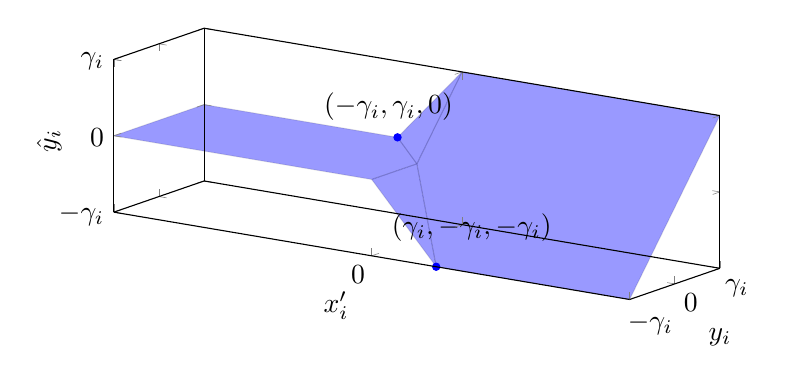
\begin{tikzpicture}[scale=0.65]
		\begin{axis}[	axis on top, xlabel = \(x'_i\),
			ylabel = {\(y_i\)}, zlabel = \(\hat{y}_i\),
			set layers=default,
			xmax = 4, xmin = -4,
			ymax = 1, ymin = -1,		
			zmax = 1, zmin = -1,
			unit vector ratio=1 1 1, scale=2.5,  ytick   = {-1,0,1},
			yticklabels = {$-\gamma_i$,$0$,$\gamma_i$}, xtick = {0},
			xticklabels = {$0$}, ztick   = {-1,0,1},
			zticklabels = {$-\gamma_i$,$0$,$\gamma_i$},
			view={35}{14},
			]
			\addplot3[ fill=blue,opacity=0.1, fill opacity=0.4] 
			coordinates {
				(0,0,0) (-1,1,0) (-4,1,0) (-4,-1,0) (0,-1,0) (0,0,0)
			};
			
			\addplot3[	fill=blue,opacity=0.1, fill opacity=0.4] 
			coordinates { (0,0,0) (0,1,1) (4, 1, 1) (4, -1, -1) (1,-1,-1) (0,0,0)
			};
			
			\addplot3[	fill=blue,opacity=0.1, fill opacity=0.4	] 
			coordinates { (0,0,0)  (-1,1,0) (0,1,1) (0,0,0)
			};
			
			\addplot3[	fill=blue,opacity=0.1, fill opacity=0.4	] 
			coordinates { (0,0,0)  (0,-1,0) (1,-1,-1) (0,0,0)
			};
			
			\addplot3[only marks, mark=*, mark size=2pt, blue] coordinates {(1,-1,-1)};
			\node[label={$(\gamma_i,-\gamma_i, -\gamma_i)$}] at (axis cs: 1.2, -0.5 ,-1) {};
			
			\addplot3[only marks, mark=*, mark size=2pt, blue] coordinates {(-1,1,0)};
			\node[label={$(-\gamma_i,\gamma_i, 0)$}] at (axis cs: -1, 0.8 ,0) {};			
		\end{axis}
	\end{tikzpicture}
	\caption{The function computing $\hat{y}_i=\ReLU(x_i)-\ReLU(x'_i)$ 
	depending on $y_i = x_i- x'_i$ and on $x'_i$.}
	\label{fig.2v}
\end{figure}
	

Recall first that we use the classical MILP encoding 
for $\hat{x}'_i=\ReLU(x'_i)$, using one binary variable $a'$. We reuse 
$a'$ (with its value already settled, see Proposition \ref{Prop1}) 
in the encoding of $\hat{y}_i = \ReLU(x_i)-\ReLU(x'_i)$:

\begin{proposition}
    \label{Prop2}
Assuming that $y_i \in [-\gamma_i, \gamma_i]$,
and that $x'_i \in [\alpha_i,\beta_i]$,
we have that $\hat{y}_i = \ReLU(x_i=x'_i+y_i)-\ReLU(x'_i)$ is the solution of:
	\begin{align*}
		& \begin{aligned}
			y_i + x'_i &\leq a\beta_i        &
			y_i &+ x'_i \geq (1-a)\alpha_i \\
			x'_i       &\leq a'\beta_i       & 
			x'_i       &\geq (1-a')\alpha_i \\
			\hat{y}_i  &\leq a\gamma_i       &
			\hat{y}_i  &\geq -a'\gamma_i \\
			\hat{y}_i  &\leq y_i + (1-a)\gamma_i  &
			\hat{y}_i  &\geq y_i - (1-a')\gamma_i \\
			\hat{y}_i  &\leq -x'_i + a\beta_i &
			\hat{y}_i  &\geq -x'_i + (1-a')\alpha_i \\
			\hat{y}_i  &\leq y_i + x'_i + (1-a)(-\alpha_i) &
			\hat{y}_i  &\geq y_i + x'_i + a'(-\beta_i)
		\end{aligned}
	\end{align*} 
    where $a,a' \in \{0,1\}$ are binary variables, 
    and $a'$ is shared with the classical MILP
    encoding for $\hat{x}'_i=\ReLU(x'_i)$.
\end{proposition}

So to encode both $\hat{y}_i$ and $\hat{x}_i$, we need 2 binary variables altogether, similar to the classical encoding.

The LP relaxation of this model contains important bounds, including 
    $\frac{y_i-\gamma_i}{2} \leq \hat{y}_i \leq \frac{y_i+\gamma_i}{2}$
    (see subsection "1v" model), which is not the case of the classical model.
	

\paragraph{A proof of Prop.~\ref{Prop2}}

We do a case analysis depending on the value of both binary variables. 
First, we know the constraints for $\hat{x_i}'=\ReLU(x_i')$ are exact (see 
Prop.~\ref{Prop1}). 

We have 2 binary variables and 4 cases in total. We only need to check that, in all 4 cases, $$\hat{y}_i = \ReLU(x'_i+y_i)-\ReLU(x'_i).$$

Case 1: if $a = 1$ and $a' = 1$, then $x'_i \geq 0 $ and $y_i+x'_i\geq 0$, then we need to show $\hat{y}_i = y_i$ based on  $\hat{x'_i} = x'_i$. This is true by the two inequalities in line 4.

Case 2: if $a = 1$ and $a' = 0$, then $x'_i \leq 0 $ and $y_i+x'_i\geq 0$, then we need to show $\hat{y}_i = y_i+x'_i$ based on  $\hat{x'_i} = 0$. This is true by the two inequalities in line 6.

Case 3: if $a = 0$ and $a' = 0$, then $x'_i \leq 0 $ and $y_i+x'_i\leq 0$, then we need to show $\hat{y}_i = 0$ based on  $\hat{x'_i} = 0$. This is true by the two inequalities in line 3.


Case 4: if $a = 0$ and $a' = 1$, then $x'_i \geq 0 $ and $y_i+x'_i\leq 0$, then we need to show $\hat{y}_i = -x'_i$ based on  $\hat{x'_i} = x'_i$. This is true by the two inequalities in line 5.

%\begin{proof}

%\end{proof}
	
	%	\begin{align*}
		%		& y_i+x'_i \leq a\beta_i \quad\wedge \quad y_i+x'_i\geq (1-a)\alpha_i\\	
		%		& x_i' \leq a'\beta_i \quad\wedge \quad x_i'\geq (1-a')\alpha_i\\
		%		&\hat{y}_i \leq a\gamma_i \quad\wedge \quad	\hat{y}_i \geq -a'\gamma_i \\
		%		&	\hat{y}_i \leq y_i+(1-a)\gamma_i \quad\wedge \quad	\hat{y}_i \geq y_i - (1-a')\gamma_i \\
		%		&	\hat{y}_i \leq -x'_i+a\beta_i \quad\wedge \quad	\hat{y}_i \geq -x'_i+(1-a')\alpha_i \\
		%		&	\hat{y}_i \leq y_i+x'_i+(1-a)(-\alpha_i)\quad\wedge \quad	\hat{y}_i \geq y_i+x'_i+a'(-\beta_i) \\
		%	\end{align*} 
	
	

	%	The relaxation of this model is similar: let $a$s and $a'$s be continuous variables instead of binary/integer variables. Unlike the first model in this section, relaxing a few nodes does not lose too much accuracy.
	
    
    
    

	\begin{figure}[b!]
		\centering
	\hspace*{10ex}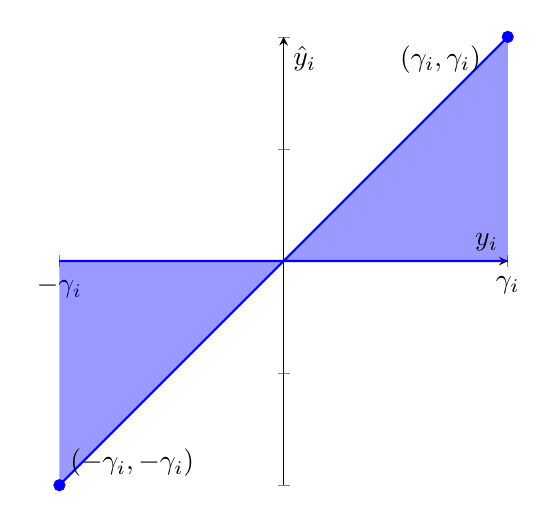
\begin{tikzpicture}
		\begin{axis}[
			xlabel={$y_i$},
			ylabel={$\hat{y}_i$},
			xmin=-2, xmax=2,
			ymin=-2, ymax=2,
			axis lines=center,
			samples=100, 
			unit vector ratio=1 1 1, scale=1, xtick   = {-2,2},
			xticklabels = {$-\gamma_i$,$\gamma_i$},
			yticklabels = {},
			]
			\addplot[blue, thick, fill=blue, fill opacity=0.4] {x} \closedcycle; 
			\addplot[blue, thick] {0}; 
			
			\addplot[only marks, mark=*, mark size=2pt, blue] coordinates {(-2,-2)};
			\node[label={above:$(-\gamma_i,-\gamma_i)$}] at (axis cs: -1.35, -2.1) {};
			
			\addplot[only marks, mark=*, mark size=2pt, blue] coordinates {(2,2)};
			\node[label={above:$(\gamma_i,\gamma_i)$}] at (axis cs: 1.4, 1.5) {};
		\end{axis}
	\end{tikzpicture}
\caption{The possible values of $\hat{y}_i=\ReLU(x_i)-\ReLU(x'_i)$ depending on $y_i = x_i-x'_i$ for the "1v" model.}
	\label{fig.1v}
\end{figure}


    \subsection{A decoupled "3v" model}

	Besides doing LP relaxation on some of the binary variables, we propose a 
    variant of the "2v" model: the binary variables $a'$ appearing in 
    Prop. \ref{Prop2} can be decoupled from the binary variable appearing in the classical encoding of $x'_i = \ReLU(x'_i)$. While this means having 3 binary variables per unstable ReLU (which warrants the name "3v" model), the fact that these variables are decouples remove a lot of constraints in the MILP encoding, and actually helps the solver. The decoupling also means that the "3v" model is not as accurate as the "2v" model.


	\subsection{The efficient "1v" model}
	
	To simplify further and limit the number of (binary) variables, 
    we introduce an efficient "1v" model which only uses the diff variables $y_i,\hat{y}_i$. Again, we study the range of values $\hat{y}_i$ can take according to the value of $y_i$, as depicted in Fig.~\ref{fig.1v}. This is a projection of Fig.~\ref{fig.2v} onto $y_i,\hat{y}_i$.
    


    \begin{proposition}
    \label{prop3}
    Given $y_i \in [-\gamma_i,\gamma_i]$, 
    $\hat{y}_i$ is a solution of the following MILP program :\begin{align*}
		\hat{y}_i &\leq a \gamma_i               &\quad \hat{y}_i &\geq y_i - a \gamma_i \\
		\hat{y}_i &\geq (a-1) \gamma_i           &\quad \hat{y}_i &\leq y_i + (1-a) \gamma_i
	\end{align*} where $a \in \{0,1\}$ is a binary variable.
	\end{proposition}

    We can easily check that the LP relaxation of this MILP program is exactly 
    $\frac{y_i-\gamma_i}{2} \leq \hat{y}_i \leq \frac{y_i+\gamma_i}{2}$, 
    {\bf LIAO please do on Fig2: as depicted in broken lines on Fig.~\ref{fig.1v}}.
    
	
	

	\iffalse
	Based on above constraints, we can sketch this simplified model:
	\begin{enumerate}
		\item For each input node, each output node, and each pre-activation and post-activation node in the hidden layers,  set one variable $y_i$. 
		\item Set constraints for input nodes.
		\item Set linear constraints . In this case, since the meaning of $y_i$ is $x_i-x'_i$, this constraints will not use the bias.
		\item Between pre- and post- activation nodes, set the MILP constraint described above.
	\end{enumerate}
	
	The key point is that, although this model sets 3 variables (and their binary variables) for each node in the network, only $y_i$  contributes to the final results, and we can ignore $x_i,x_i'$ (and their binary variables) during the optimization.
	
	As a result, we can relax the binary variables used to $\hat{x}_i = \ReLU(x_i)$ and $\hat{x}'_i = \ReLU(x'_i)$.
	\fi

	The "1v" model contains the same number of (binary) variables as the MILP model for local robustness, but it is not as accurate as the "3v" or "2v" models. 
    
	%	However, in practice, with a reasonable timeout, this simplified model can usually obtain a better bound.
	%	


    
	
	\subsection*{A trick of $L_1$ norm constraints on input}

A trick to set $L_1$ norm constraints on the input space into linear constraints is described below.

Suppose the dimension of input space is $n$, and $x_i,i\leq n$ are the input variables, $\vec{x}$ is the input vector, and we hope to set a constraints of $\vec{x}$ that $\|\vec{x}\| \leq c$,  then we can set the constraints by add variables $A_i,i<n$ with the only constraints \begin{align}\label{L1constraint}\begin{cases}
	A_i \geq x_i &\text{ for }i \leq n\\ 
	A_i\geq -x_i &\text{ for }i \leq n\\
	\Sigma_{i\leq n} A_i \leq c	&\end{cases}
\end{align}

We show that this constraint is equivalent to $\|\vec{x}\| \leq c$.

The first two lines of constraints \ref{L1constraint} is equivalent to that $A_i\geq |x_i|$. So the whole constraints is non-weaker than $\|\vec{x}\| \leq c$.

Next, for every instance that satisfy $\|\vec{x}\| \leq c$, then there is also an instance which satisfy constraints \ref{L1constraint}: simply let all $A_i = |x_i|$. And this shows that $\|\vec{x}\| \leq c$ is non-weaker than constraints \ref{L1constraint}. Therefore they are equivalent.

	
	\newpage
	
	\newpage

\section{Experimental Evaluation}


We implemented a prototype of \toolname in Python 3.8. 
We conducted our evaluation on an AMD 5975WX  ($32$ cores$@3.6$GHz, 7nm, year 2022) 
with 256 GB of main memory and 2 NVIDIA RTX 3090. 
Gurobi 9.52 was used for solving MILP and LP problems. 

We conducted our evaluation on neural networks trained on MNIST that have been employed in prior work. The networks have varying sizes: $5\times 100$, $5\times 200$, $8 \times 100$, and $8 \times 200$. It is worth remarking that despite seemingly small size, these instances are challenging for the current state of the art techniques. In particular, the current state of the art methods are unable to characterize $12\%$ to $20\%$ of the images as neither certified robust \cite{crown} nor find an adversarial example \cite{attack}. We call such images {\em undetermined}. Following methodology in prior work \cite{prima,crown}, we evaluate on the first 1000 images of the dataset. We also experimented on the network of size $6\times 500$ (results not reported in \cite{prima,crown}), checking the first 200 images of the dataset, given the computational overhead associated with such larger networks. 
Each DNN is associated with a $\varepsilon>0$ for the $L^\infty$ norm.
All these DNNs are found in the ERAN GitHub 
(\url{https://github.com/eth-sri/eran}, the 4th to the 8th DNNs provided).
%Each DNN is associated with a $\varepsilon>0$ for the $L^\infty$ norm.

\paragraph{Baseline}: 
We compare the following verifiers performing value-abstraction:
\begin{itemize}
	\item DeepPoly \cite{deeppoly}/ CROWN \cite{crown}. We report the runtime from our own implementation, used in {\toolname}. It shows that our purely Python implementation is not optimal ($10$ to $100$ times slower than the implementation in ($\alpha$)($\beta$)CROWN, ERAN and PRIMA). 
	\item PRIMA~\cite{prima} and $(\alpha)\beta$ CROWN \cite{crown}. We use the results reported in \cite{prima} and \cite{crown} respectively for instances that were also used in prior works.
	We report results for the $6\times500$ network as it was not reported in prior work.  
	
%	They use GPU while we do not. When computing the whole correlated space, 
%	parallelization is difficult.
%	Notice that on these DNNs, PRIMA resort to refined bounds on the first few layers (3 or 4) using exact MILP encoding of all the nodes (which is easily parallelized - 16 nodes considered in parallel in PRIMA). This is doable on the first few layers as the number of integer variable is not too large. By comparison, we run MILP on all the layers, but with a bounded number of integer variables to control the runtime and to scale to all the layers.
%	Its main idea is to implement a very efficient Branch and Bound (BaB) verification tool, subsuming BaBSR \cite{BaB}, and using GPU implementation (while we do not). Performance of pure BaB on these 
%	"hard to verify" DNNs is however impaired by the large number of branchs to consider. Similarly as PRIMA, $\beta$-CROWN resorts to refining the bounds of the first few layers using an exact MILP encoding, also computing 16 nodes in parallel, before running the branching heuristic BaB-FSB. 
%	\item We also experimented with the latest versions of $\alpha$-$\beta$-CROWN (October 2023) and PRIMA (2022) on MLP $6 \times 500$ (results not reported in \cite{crown,prima}).
	\item It is worth remarking that we do not report results from kPoly \cite{kpoly}, OptC2V \cite{optC2V}, 
	SDPFO \cite{SDPFI}, MIPplanet \cite{MIPplanet}, as $(\alpha)\beta$-CROWN has been shown to outperform these methods \cite{crown}.
	
\end{itemize}



The  objective of our evaluation was to answer the following  questions:

\begin{enumerate}
	\item How does the the choice of  the set  $Z$ impacts the accuracy of $\MILP_Z$? 
	\item  How does the performance, measured as the percentage of images verified, of \toolname compare to that of prior state of the art approaches? 
%	\item Evaluate how the runtime of \toolname scales with the size of DNNs.
\end{enumerate}

\subsection{Utility of Heuristic based on Compensation Strength  }

%The first group of experiments we run, tests the accuracy of choosing a set $Z$ of $K$ nodes using compensation strength, compared with randomly choosing the same number $K$ of nodes,  to understand if the choice is meaningful or any set $Z$ with the same size will result in a similar accuracy.
To measure the impact of the heuristic based on compensation strength, we focused on the smallest DNN (i.e. of size $5\times 100$ \cite{crown}) so as to obtain exact bounds for the first few layers using a full MILP encoding of the DNN. We test over the $\vx=59$th image in the MNIST dataset, as it has a large number of unstable ReLU nodes in the first few layers ($61$ in the first and $55$ in the second layer), so we can experiment with a larger choice of values) for $K$.

To measure the accuracy, we measure the uncertainty of all nodes in a layer:
the uncertainty of a node is the range between its computed lower and upper bound. 
We then average the uncertainty among all the nodes of the layer.
Formally, for a node $n$ with bounds $[\alpha,\beta]$, its uncertainty $unc(a) = \beta - \alpha$, and the average uncertainty of a layer $l$ is $\dfrac{\sum_{a\in l} unc(a)}{|l|}.$







%KSM: I don't think this is really the place for the paragraph below
% Let $c$ be a node of the second layer.
%A compensating pair $(\pi,\pi')$ of paths with target $c$ is thus of the form a node $a b c$ and $a b' c$, with $a$ an input node and $b,b'$ on the first layer. The compensating strength for $(b,b')$ is defined as $comp(b,b')=\sum_a \val_{\vx}(a) \min(weight(abc),weight(ab'c))$. Indeed, the pair $(a b c,a b' c)$ of path cannot compensate more than $\val_{\vx}(a) \min(weight(a,b,c),$\newline $weight(a,b',c))$, and $b,b'$ would help compensated the set of pairs of paths $\{(a b c,a b' c) \mid a$ is in the first layer$\}$. After selecting the heaviest $(b_0,b_0')$, we can then compute $comp(b)= \sum_{b' \text{already selected}} comp(b,b')+comp(b',b)$ and select iteratively the heaviest $b$'s one by one till reaching the threshold. 
%We do this for all node $c$ of the second layer.



\subsubsection*{ReLU Node in the first hidden layer}


We first focus on the choice of nodes in the first hidden layer, and its consequences on the accuracy of nodes in the second layer. 
We report in Table \ref{tab:example0} the average uncertainty of $\MILP_Z$ following the choice of the $K$ heaviest compensating ReLU nodes in $Z$, vs choosing $K$ nodes randomly. The range of uncertainty created by inacurate computations is up to $1.17=2.22-1.05$, $2.22$ being the accuracy provided by LP, and $1.05$ by an exact MILP encoding of all the unstable ReLU nodes. Selecting $30$ out of the $61$ unstable ReLU nodes, the uncertainty created by inacurracies is reduced by $80\%$, while a random choice of nodes only leads up to roughly halving this number. We can deduce that selecting nodes based on compensating strength helps to select important ReLU nodes for the accuracy.



\begin{table}[h!]
	\centering
	\begin{tabular}{|c||c|c|}
		\hline
		\text{Number $K$ of nodes in $Z$}  &  \text{Compensate strength} & \text{Random Choice}  \\ \hline
		\hline
		0  &  2.22 & 2.22  \\ \hline
		10  &  1.84 & 2.03  \\ \hline
		20  &  1.50 & 1.82  \\ \hline
		30  &  1.28 & 1.62  \\ \hline
		40  &  1.14 & 1.44  \\ \hline
		50  &  1.06 & 1.23  \\ \hline
		61 (max) & 1.05 &  1.05 \\ \hline
	\end{tabular}
	\caption{Average uncertainty of $\MILP_Z$ for nodes of the second layer, for $Z$ with $K$ ReLU nodes of the first layer (compensating strength vs random choice).}
	\label{tab:example0}
	%\vspace{-0.8cm}
\end{table}


{\color{red} We also do a comparison of our method and the method in paper \cite{9211410}. They find a formula to choose nodes in their algorithm. We can use the same formula in our setting, and since we only have $\ReLU$ function, that formula can be simplified to: $$V(n) = (UB(n)-LB(n))\cdot W_{nm}.$$ In this formula, $m$ is the target node, and $n$ is one of source nodes in one layer before. We sort all nodes $n$ by their $V(n)$ values, and choose the nodes with largest values.}

\subsubsection*{ReLU Node in the first and second hidden layer}

We now turn to evaluating the choice of ReLU nodes in two layers, focusing on the uncertainty of nodes in the third layers, wrt ReLU nodes in the first and second layer.
The bounds for nodes of the first two layers are computed exactly using the full MILP encoding. Let $d$ be a neuron of the third layer.
We keep the previous evaluation for ranking nodes in the previous (second) layer. 
Once the set $Z$ of selected nodes has sufficiently many nodes $c,c'$ in the second layer, adding $b,b'$ from the first layer to $Z$ allows to take into account accurately the pairs of paths of the form $(a b c d, a b' c' d)$ for all $\{c,c'\} \in Z$. We thus define:
%\vspace{-0.2cm}
$$comp(b,b')=\sum_a \sum_{c,c' \in Z} \val_{\vx}(a) \min( weight(abcd),weight(ab'c'd))$$ and the associated $comp(b)=\sum_{b' \in Z} comp(b,b') + comp(b',b)$. We then select iteratively nodes $b$ (first layer) or $c$ (second layer) by selecting the heaviest $comp(b)$ or $comp(c)$. {\color{red} The intuition behind the formula is straightforward: $\val_{\vx}(a)weight(abcd)$ is the simple contribution from node $a$ to the target $d$. And min of two paths is a natural value to represent the strength of compensation: if one of them is very small, the effect of compensation will also be very small.}

We report in Table \ref{tab:example1} the average uncertainty of $\MILP_Z$ following the choice of the $K$ heaviest compensating ReLU nodes in $Z$, vs choosing $K$ nodes randomly from layers $1$ and $2$. 
We compare choosing nodes in the second layer only with choosing nodes in both the first and second layer.
Choosing ReLU nodes in the previous layer (layer $2$) only is less accurate than 
also choosing nodes in layer $1$. When picking in both layer $1$ and $2$, choosing $50$ out of $116$ unstable ReLU nodes allows to reduce by $90\%$ the average uncertainty due to inaccurate computations ($0.059$ vs $0.574$), while it only reduces the uncertainty by $65\%$ when choosing nodes randomly. Notice that applying this layer after layer will even further reduce uncertainty created by accumulation of inaccuracies. 
Last, we did not experiment for selecting ReLU nodes in 3+ layers earlier because the trade-off of accuracy vs evaluating the compensating strength of such paths is unclear.

\begin{table}[t!]	
	\centering
	\begin{tabular}{|c||c|c|c|}
		\hline
		\text{Number $K$}  &  \text{Compensate layer} 1+2 &  \text{Compensate layer} 2 & \text{Random layer } 1+2 \\ \hline
		\hline
		0  &  1.761 & 1.761 & 1.761  \\ \hline
		10  &  1.656 & 1.651 & 1.696  \\ \hline
		20  &  1.527 & 1.557 & 1.619  \\ \hline
		30  &  1.402 & 1.489 & 1.546  \\ \hline
		40  &  1.281 & 1.447 & 1.469  \\ \hline
		50  &  1.165 & 1.426 & 1.388  \\ \hline
		116 (max) &  0.895 & 1.424 & 0.895  \\ \hline
	\end{tabular}
	\caption{Average uncertainty of $\MILP_Z$ for nodes of the third layer, for $Z$ with $K$ ReLU nodes of the 1st and 2nd layer (compensating strength vs random choice).}
	\label{tab:example1}
	\vspace{-0.6cm}
	
\end{table}

\subsection{Comparison with Prior State of the Art}

We present the runtime and accuracy analysis of various techniques in Table~\ref{tab:example}. Further, for each DNN, a PGD-attack \cite{attack} is run 
on all the images. We report the $\%$ of images without attack, as being an {\em Upper Bound} on the $\%$ of images the vertifiers can certify.

Several observations are noteworthy: DeepPoly (or CROWN) is by far the fastest, yet it is also the least accurate, certifying robustness for fewer than $30\%$ of the images. In contrast, there are at least $82\%$ of the images for which no attack is found. Similarly, PRIMA achieves better accuracy than DeepPoly/CROWN but falls short of \toolname. 

Next, we shift focus to the comparison with ($\alpha$)$\beta$-CROWN, where we observe intriguing trade-offs. On the shallowest DNNs (5 layers, $5 \times 100$, $5 \times 200$), \toolname accuracy is close to $\beta$-CROWN, within 1.5\%. Here, RefinedBaB used by $\beta$-CROWN, has the time to refine most of the nodes, and thus the number of branches BaB has to explore is small enough that its very accurate.

As network sizes increase, \toolname demonstrates better accuracy in comparison to $\beta$-CROWN. For instance, for $8 \times 100$ and $8 \times 200$, 
RefinedBaB used by $\beta$-CROWN can only consider half of the layers. 
On many images, there are too many branches for BaB left to consider, and it times out,
reason why we close the gap of undetermined images from $17.6\%$ ($\beta$-CROWN) to $10.4\%$ (\toolname) in $8 \times 200$. 

As expected, there's a trade-off between runtime and accuracy: \toolname can verify more images, albeit at the cost of increased computation time. However, more often than not, our primary concern lies in running a tool to determine whether it can verify the desired property within a reasonable time.


The last network $6 \times 500$ (trained naturally) is the largest one. Results were not reported in \cite{crown,prima}. On this larger network, the refined strategy of PRIMA and $\alpha,\beta$-CROWN is questionable, as the number of binary variables to encode even the first few layers is very large, and the efficiency of MILP unclear. As a matter of fact, refinedBaB is "NotImplemented" in $\alpha,\beta$-CROWN for this network, and the results are 
surprisingly inaccurate and fast in PRIMA (even faster than for $5 \times 100$), probably because few/no nodes are actually refined. We reported the standard pureBaB setting of $\alpha,\beta$-CROWN instead, with the usual 30s associated timeout. Accuracy on $\alpha,\beta$-CROWN was also very low, only $15\%$ more images verified than DeepPoly. To understand the impact of runtime, we also experimented with a 2000s timeout for $\alpha,\beta$-CROWN. It only improves the accuracy by $3.5\%$, at $44.5\%$, with a runtime of $954s$ ($50$ times longer than with the original $30s$ timeout). We conclude that the number of branches is often too high for $\alpha,\beta$-CROWN to tackle such a hard DNN.
For comparison, \toolname could verify more than $20\%$ more images than
even $\alpha,\beta$-CROWN with the longest timeout, taking less than $0.3s$ per neuron to perform the verification in average per image.




% BaB focuses on the output neuron, computing bounds for it, and refining the different ReLU as necessary. Instead, we consider every node one by one from the input layer till the final layer, with the same accuracy. Hence {\toolname} will spend a lot of time on nodes which are not necessary for the verification. 
% 
%It is worth remarking that our prototype implementation (in Python)  Therefore, our naive implementation is not as efficient as the highly optimized $\beta$-CROWN: our slow setting is $1.4$ to 
%$6.5$ times slower than $\beta$-CROWN. Notice {\toolname} it is not using GPUs. 
%Concerning accuracy: on shallower DNNs ($5 \times 100$ and $5 \times 200$ with $5$ hidden layers), refined BaB uses MILP on all but the last $2$ layers, leaving BaB with few ReLU nodes to branch on, and $\beta$-CROWN (refined BaB) is slightly more accurate than using the slow fixed setting of {\toolname}, with a small difference of less than $1.5\%$. On deeper DNNs ($8 \times 100$ and $8 \times 200$ with $8$ hidden layers), the full MILP used in refined BaB cannot treat the last $4$ layers, and BaB has more ReLU nodes to branch on: 
%the most accurate setting (slow fixed) of {\toolname} is more accurate than $\beta$-CROWN, closing the gap with the upper bound from $20\%$ to $16.2\%$ ($8 \times 100$)
%and from $17.6\%$ to $10.4\%$ ($8 \times 200$). This is very promising for the compensation idea, which could be used in many different ways than in {\toolname} (see Section \ref{Discussion}).

%Further, unlike PRIMA, we do not resort to a GPU, and our purely Python implementation is not optimal. This is very promising for this idea of compensation, which indirectly treats dependencies between the variables, which PRIMA represents explicitly.





%In Table \ref{tab:example}, we report the accuracy and runtime of these different methods.
%DeepPoly/CROWN is by far the fastest, but also the most inaccurate, certifying robustness for less than $30\%$ of the images, whereas there are at least $82\%$ of the images for which no attacked is found (attacks computed by \cite{attack} in $\beta$-CROWN).
%This is because these DNNs, although of reasonable size, are hard to verify (they are trained in a natural way, with high compensation strength, see Section \ref{Sec.comp}).


%Compared with PRIMA (using refinement of the first few layers by exact MILP), the overall pipeline is quite similar, looking at all the nodes one by one from the beginning of the network till the end. 
%Now, moving on to PRIMA, our 
%Our method compare favorably, both in terms of time and accuracy: our fast adaptive setting is always faster than PRIMA, sometimes by a large margin ($>3$ times faster on $8 \times 100$ while verifying $10\%$ more images), and also more accurate (except for $5 \times 200$ which is quite pointless on this shallow DNN - the fast fixed method is both faster and more accurate than PRIMA), sometimes by a large margin (by $14 \%$  for $5 \times 100$ while being $30\%$ faster). Further, unlike PRIMA, we do not resort to a GPU, and our purely Python implementation is not optimal. This is very promising for this idea of compensation, which indirectly treats dependencies between the variables, which PRIMA represents explicitly.

\newcolumntype{C}{>{\centering\arraybackslash}X}


\begin{table}[t!]
	\centering
	\begin{tabularx}{\textwidth}{|C||C||C|C|C||C|}
		
		\hline
		\text{DNN} & \shortstack{Upper\\Bound} & \shortstack{DeepPoly/\\CROWN} & PRIMA & \shortstack{($\alpha$)$\beta$-\\CROWN} & \toolname \\ 
		\hline \hline
		
		$5 \times100$\  & $84.2 \%$ & $16\%$ & $51\%$ & $\mathbf{69.9\%}$ & $68.4\%$\\ 
		$\epsilon = 0.026$ &  & 5s & 159s & 102s & 142s\\
		\hline	
		
		$5 \times 200$ \  & $90.1 \%$ & $18.2\%$ & $69\%$ & $\mathbf{77.4\%}$ & {$76.8\%$}\\ 
		$\epsilon = 0.015$ &  & 11s & 224s & 86s & {279s} \\ \hline \hline
		
		
		$8\times100$\  & $82.0 \%$ & $29.2\%$ & $42.8\%$ & $62\%$ & {$\mathbf{65.8\%}$}\\ 
		$\epsilon = 0.026$ &  & 8s & 301s & 103s & {346s}\\
		\hline
		
		$8\times200$\  & $91.1 \%$ & $25.9\%$ & $62.4\%$ & $73.5\%$ & {$\mathbf{80.7\%}$}\\ 
		$\epsilon = 0.015$ &  & 17s & 395s & 95s  & {697s}\\ \hline \hline
		
		$6\times500$\  & $92\%$ & $26\%$ & $32.5\%$ & $41\%$ & {$\mathbf{65\%}$}\\ 
		$\epsilon = 0.035$ &  & 34s & 119s & 18.4s & {925s} \\ \hline 
		
	\end{tabularx}
	
	\caption{$\%$ of verified images and average runtime in seconds.
		Results for PRIMA, $\beta$-Crown and the upper bound on the $\%$ are from \cite{crown}.
	}
	\vspace{-0.8cm}
	\label{tab:example}
\end{table}







%\begin{table}[t!]
%	\centering
%	\begin{tabular}{|c||c|c|c||cc|cc||c|}
%		
%		\hline
%		\text{DNN}  & DeepPoly & PRIMA & $\beta$-CROWN &\multicolumn{2}{@{}c@{}|}{\color{blue}\text{ Comp (adapt.) }} & \multicolumn{2}{@{}c@{}|}{\color{blue} \text{ Comp (fixed) }} & Upper\\ 
%		& / CROWN & (refined) & (refined BaB) & {\color{blue}fast} & {\color{blue}slow} & {\color{blue}fast} &{\color{blue}slow} & Bound\\
%		\hline \hline
%		
%		$5 \times100$\  &   $16\%$ & $51\%$ & $\mathbf{69.9\%}$ & {\color{blue}$57.5\%$} & {\color{blue}$66.1\%$} & {\color{blue}$65.3\%$} & {\color{blue}$68.4\%$} &  $84.2 \%$ \\ 
%		$\epsilon = 0.026$ & 5s & 159s & 102s& {\color{blue}75s} & {\color{blue}140s} & {\color{blue}117s} & {\color{blue}142s} &  \\
%		\hline	
%		
%		$5 \times 200$ \  &  $18.2\%$ & $69\%$ & $\mathbf{77.4\%}$ & {\color{blue}$64.3\%$} & {\color{blue}$74.7\%$} & {\color{blue}$72\%$} & {\color{blue}$76.8\%$} & 
%		$90.1 \%$\\ 
%		$\epsilon = 0.015$ & 11s & 224s & 86s & {\color{blue}163s} & {\color{blue}285s} & {\color{blue}206s} & {\color{blue}279s}  &\\ \hline \hline
%		
%		
%		$8\times100$\  &   $29.2\%$ & $42.8\%$ & $62\%$ & {\color{blue}$52.7\%$} & {\color{blue}$59.7\%$} & {\color{blue}$61.4\%$} & {\color{blue}$\mathbf{65.8\%}$}  & $82.0 \%$ \\ 
%		$\epsilon = 0.026$ & 8s & 301s & 103s & {\color{blue}92.3s} & {\color{blue}179s} & {\color{blue}170s} & {\color{blue}346s} & \\
%		\hline
%		
%		
%		$8\times200$\  &   $25.9\%$ & $62.4\%$ & $73.5\%$ & {\color{blue}$68.1\%$} & 
%		{\color{blue}$79.1\%$} & {\color{blue}$72.6\%$} & {\color{blue}$\mathbf{80.7\%}$} & $91.1 \%$ \\ 
%		$\epsilon = 0.015$ & 17s & 395s & 95s  & {\color{blue}297s} & {\color{blue}535s} & {\color{blue}$480s$} & {\color{blue}697s$^\star$} & \\ \hline
%		
%		%6$\times$500\  &   0.035& 1.758 & time & 1.758 & time &    1.758 & time & 1.758 & time & \\ 
%		%$\epsilon = 0.035$ & & & & & & & & & &\\ \hline
%	\end{tabular}
%	\caption{$\%$ of verified images and average runtime in seconds, over 1000 images. 
%		Results for PRIMA, $\beta$-Crown and the upper bound on the $\%$ are from \cite{crown}.
%		\newline $^\star$ For $8 \times 200$, slow fixed results are obtained after running slow adaptative.}
%	\label{tab:example}
%%	\vspace{-1cm}
%\end{table}


%Compared with $\beta$-CROWN (also using a refinement on the first few layers using exact MILP), the picture is more balanced, because the fundamentals of both algorithms are different. BaB focuses on the output neuron, computing bounds for it, and refining the different ReLU as necessary. Instead, we consider every node one by one from the input layer till the final layer, with the same accuracy. Hence {\toolname} will spend a lot of time on nodes which are not necessary for the verification. Therefore, our naive implementation is not as efficient as the highly optimized $\beta$-CROWN: our slow setting is $1.4$ to 
%$6.5$ times slower than $\beta$-CROWN. Notice {\toolname} it is not using GPUs. 
%Concerning accuracy: on shallower DNNs ($5 \times 100$ and $5 \times 200$ with $5$ hidden layers), refined BaB uses MILP on all but the last $2$ layers, leaving BaB with few ReLU nodes to branch on, and $\beta$-CROWN (refined BaB) is slightly more accurate than using the slow fixed setting of {\toolname}, with a small difference of less than $1.5\%$. On deeper DNNs ($8 \times 100$ and $8 \times 200$ with $8$ hidden layers), the full MILP used in refined BaB cannot treat the last $4$ layers, and BaB has more ReLU nodes to branch on: 
%the most accurate setting (slow fixed) of {\toolname} is more accurate than $\beta$-CROWN, closing the gap with the upper bound from $20\%$ to $16.2\%$ ($8 \times 100$)
%and from $17.6\%$ to $10.4\%$ ($8 \times 200$). This is very promising for the compensation idea, which could be used in many different ways than in {\toolname} (see Section \ref{Discussion}).


%KSM: I think this paragraph doesn't make very convincing case. 
%Importantly, ($\alpha$)$\beta$-Crown, while efficient, can face a (complexity) wall, when the number of branches becomes too extreme for BaB to work: either BaB succeds fast, or it will not suceed even with very long timeouts ({\em refined} BaB is more accurate than pureBaB on these networks). We verify that in Table \ref{tab:example3}, on a larger DNN learnt in a natural way, namely MLP $6 \times 500$.
%We tested PureBaB with two timeouts (TO), from standard 30s to an extreme 2000s, to match the average runtime of our adaptative implementation (fast mode). Only $3.5\%$ more images could be ceritifed by extending the TO from 30s to 2000s, certifying $20\%$ less images than our prototype in the same time. Notice that the refined BaB mode of ($\alpha$)$\beta$-Crown (first few layers using MILP) failed to run on this DNN (error code: NoImplementation), and we were unable to fix the problem, which is not really surprising as running exact MILP with so many integer variables is not likely to be efficient, as confirmed while running PRIMA (refined).



% test

%
%\begin{table}[t!]
%	\centering
%	\begin{tabular}{|c||c|c|cc||c||c|}
%		
%		\hline
%		\text{DNN}  & DeepPoly & PRIMA &  \multicolumn{2}{@{}c@{}|}{\text{ $\alpha$-$\beta$-CROWN (pureBaB) \,}} & 
%		{\color{blue}Comp (adapt.)} & Upper\\ 
%		& / CROWN & (refined) & TO=30s & TO=2000s & {\color{blue}fast} & Bound\\
%		\hline \hline
%		$6\times500$\  &   $26\%$ & $32.5\%$ & $41\%$ & $44.5\%$  & {\color{blue}$\mathbf{65\%}$} & $92\%$ \\ 
%		$\epsilon = 0.035$ & 34s & 119s & 18.4s & 954s & {\color{blue}925s} &\\ \hline
%	\end{tabular}
%	\caption{$\%$ of verified images and average runtime in seconds, over 200 images.}
%	\label{tab:example3}
%	
%\end{table}

%\begin{table}[]
%	\centering
%	\begin{tabular}{|c|c|cc||cc||c|}
%		\hline
%		\text{DNN}  & DeepPoly &  \multicolumn{2}{@{}c@{}|}{\text{ $\alpha$-$\beta$-CROWN (refinedBaB) \,}} & 
%		\multicolumn{2}{@{}c@{}|}{\text{ \color{blue}\CMP slow \,}}
%		& Upper\\ 
%		& / CROWN & TO=300s & TO=3000s & {\color{blue}adapt} & {\color{blue}fixed} & Bound\\
%		\hline \hline
%		$8\times200$\  &   $25\%$? & $72\%$? & $\mathbf{79.5\%}$ & {\color{blue}$75.5\%$}  & {\color{blue}$77\%$} & $91\%$ \\ 
%		$\epsilon = 0.015$ & 17s & 95s? & 451s & {\color{blue}391s} & {\color{blue}562s} &\\ \hline
%	\end{tabular}
%	\caption{WIP! $\%$ of verified images over 200 images. To see how refined BAB scale with TimeOut.}
%	\label{tab:example4}
%\end{table}


\iffalse

\subsection{Scalability of {\toolname} with Size of DNNs}

\begin{figure}[b!]
	\centering
	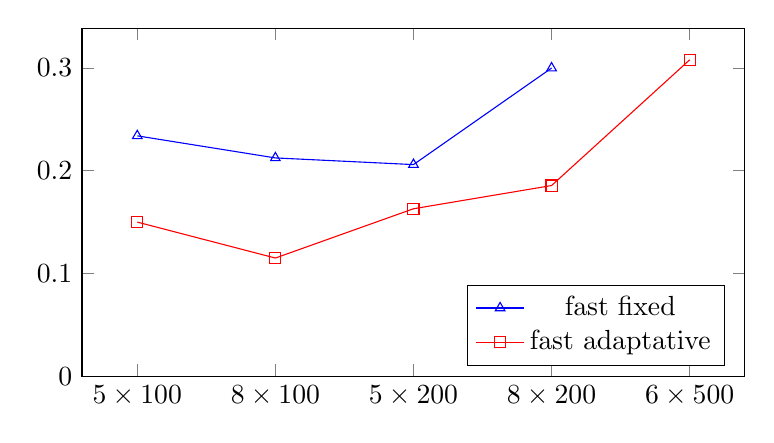
\begin{tikzpicture}
		\begin{axis}[width=10cm,height=6cm,
			xlabel={},
			ylabel={},
			legend pos=south east,
			ymin=0,
			xtick={1,2,3,4,5}, 
			xticklabels={$5\times 100$, $8\times 100$, $5\times 200$, $8\times 200$, $6\times 500$},
			]
			
			
			\addplot[mark=triangle, blue] coordinates {
				(1, 0.234)
				(2, 0.2125)
				(3, 0.206)
				(4, 0.3)
			};
			\addlegendentry{fast fixed}
			
			
			\addplot[mark=square, red] coordinates {
				(1, 0.15)
				(2, 0.115)
				(3, 0.163)
				(4, 0.1856)
				(5, 0.308)
			};
			\addlegendentry{fast adaptative}
			
			
		\end{axis}
	\end{tikzpicture}
	\caption{runtime (seconds per node)}
	\label{fig2}
\end{figure}



We now focus on understanding the potential of {\toolname} for even larger networks than those that are usually considered in the verification community. To this end, Figure~\ref{fig2} presents the  average runtime per node across various DNNS. Observe that while  the average runtime per node isn't fixed (attributable to $\LP(N,K)$), it remains regulated, avoiding exponential increases — from 0.1s per node for the smallest DNN to 0.3s per node for the largest. This suggests that {\toolname} is scalable to larger DNNs, bypassing the high complexity barrier often encountered with approaches such as those based on pure branch and bound.

\fi


\section{Discussion}
\label{Discussion}


In this work, we focused on DNNs employing ReLU activation functions since our approached on usage of MILP, which is naturally suited for ReLU activation function. However, it is worth remarking that the notion of compensation strength is independent of  activation function, and therefore, an interesting direction of future work would be to explore other the impact of compensation strength-based approaches for other activation functions. 


Regarding accuracy, {\toolname} ranks highly among verifiers that abstract values. However, its runtime, particularly for larger DNNs, can be relatively slow, though not excessively so. Numerous optimization avenues exist. A primary strategy involves utilizing $\alpha$-$\beta$-CROWN initially in the sequence, reserving {\toolname} for images unresolved by $\alpha$-$\beta$-CROWN, potentially enhancing this with parallel node computation across additional CPU cores. Another tactic could involve adapting the refined branch-and-bound approach of $\beta$-CROWN to permit {\toolname} to process additional layers beyond MILP's capability, concluding the verification with BaB. More complex strategies might include modifying BaB to branch on unstable ReLU nodes, driven by compensation strength, or analyzing crucial nodes linked to uncertain outputs, enabling quicker computation of less precise bounds for less critical nodes. Furthermore, implementing a Refinement Abstraction framework, akin to methodologies in \cite{atva}, \cite{elboher}, or \cite{SRGR}, could be beneficial.


In terms of neuron correlation, a key feature explicitly encoded by PRIMA, our findings suggest that leveraging compensation strength for network abstraction is generally more effective. Although precise local accuracy is achieved by directly considering ReLU nodes, the accuracy diminishes when correlations originate from distant layers. Retaining a select few significant correlations, in the style of PRIMA, as explicit linear constraints in the MILP model, might offer a strategy to further improve accuracy. 






	%\vspace{-0.5cm}
	\section{Related Work}

Some works \cite{Leino,Zhang22a,Sun22,Chen21,REGLO} focus on training a network to be - rather than proving the DNN is - globally robust.
Other works \cite{Bastani16,Ruan19,Gopinath18} estimate global robustness bounds, but without hard verification certificates, e.g. using probabilistic guarantees 
\cite{Levy23,Mangal19}.

Closer to our paper, several works  \cite{Marabou,lipshitz,ITNE,GROCET} consider a global certified restricted Lipschitz bound, to understand how the output change with input perturbations. However, they do not consider whether the classification changes. 

The most related work is Vhagar \cite{vhagar}, which also computes $\beta^\varepsilon_{i,j}$ bounds, but limited to $L_\infty$-perturbations (and variants). They do not however report {\em real-time} certified robust percentage, as in Table \ref{table.cert}. Last, their hyper-adversarial attack to find better lower bounds seems very efficient, and we will consider it in the future.

Technically, none of the MILP base work \cite{vhagar,lipshitz,ITNE} 
consider $L_1$-perturbations. Further, they use the classical MILP encoding from \cite{MILP}, and not our novel "2v" model, nor even our "1v" model. However, \cite{ITNE} 
defines the {\em diff variables} $y,\hat{y}$, adding explicitly the linear relaxation $\frac{y_i-\gamma_i}{2} \leq \hat{y}_i \leq \frac{y_i+\gamma_i}{2}$ implied by our models, Eq. (3) in \cite{ITNE} corresponding essentially to it. \cite{vhagar} does things differently, adding per neuron constraints (depending on the perturbation) between the (binary) variables to simplify the MILP problem, which is well-adapted to occlusion and patches but less to $L_1$-perturbations. 


	
	
	
\section{Conclusion}

In this paper, we introduced a novel "2v" MILP model for global verification questions, which is 4 to 8 times more accurate than the classical MILP model,
and more accurate than the ITNE model of \cite{lipshitz}, see 
Table \ref{table.classical}. Using our "3v" or "1v" models abstracting away some features of the "2v" model,
 even better bounds are reached (Tables 3, 4, 5). We also explained how to support $L_1$-perturbations efficiently on top of classical $L_\infty$-perturbations (Prop \ref{prop.l1}). To further lower the bounds by $> 10$ times, we resort to model order reduction, reducing the space of search closer to the space of the training dataset, without sacrificing DNN accuracy ($97\%$). This results into, to the best of our knowledge, the first {\em real-time} robustness certification reported for a DNN, with $86\%$ of robustness for an $L_1$-perturbation of $.5$ and $53\%$ of robustness for an $L_1$-perturbation twice as large of $1$. Still, global verification is only at its beginning, and combining different methods is necessary to scale to more complex DNNs.

	
	
	
	
	 
	
	
	\newpage

	
	\bibliography{references}
	
	
\end{document}
